\setcounter{chapter}{3}

\chapter{Categorial Explanatory Variables}


{\small \textit{Chapter Preview}. \textit{Categorical variables}
allow us to group observations into distinct categories. This
chapter shows how to incorporate categorical variables into
regression functions using binary variables, thus considerably
widening the scope of potential applications for regression
analysis. Statistical inference for several coefficients is
introduced in this chapter to allow analysts to make decisions about
categorical variables (as well as other important applications).
Categorical explanatory variables also provide the basis of
\textit{ANOVA} models, representations which are equivalent to
regression in some circumstances that permit easier interpretation
and analysis.}

\section{The Role of Binary Variables}\label{S4:BinaryVar}

\marginparjed{Categorical variables provide labels for observations
to denote membership in distinct groups, or categories.}

\textit{Categorical variables} provide labels for observations to
denote membership in distinct groups, or categories. A binary
variable is a special case of a categorical variable. To illustrate,
a binary variable may tell us whether or not someone has health
insurance. A categorical variable could tell us whether someone has
\begin{itemize}
\item private group insurance (offered by employers and
associations), \item private individual health insurance (through
insurance companies), \item public insurance (such as Medicare or
Medicaid) or \item no health insurance.
\end{itemize}

\noindent For categorical variables, there may or may not be an
ordering of the groups. In health insurance, it is difficult to
order these four categories and say which is ``larger,'' private
group, private individual, public or no health insurance. In
contrast, for education, we might group individuals into ``low,''
``intermediate'' and ``high'' years of education. In this case,
there is an ordering among groups based on level of educational
achievement. However, as we will see, this ordering may or may not
provide information about the dependent variable. \textit{Factor} is
another term used for an unordered categorical explanatory variable.

\marginparjed{Factor is another term used for an unordered
categorical explanatory variable.}

For ordered categorical variables, analysts typically assign a
numerical score to each outcome and treat the variable as if it were
continuous. For example, if we had three levels of education, we
might employ ranks and use
\begin{equation*}
\textrm{EDUCATION} = \left\{ \begin{array}{cl}
        1           & \textrm{for low education} \\
        2           & \textrm{for intermediate education} \\
        3           & \textrm{for high education.} \\
\end{array} \right.
\end{equation*}
An alternative would be to use a numerical score that approximates
an underlying value of the category. For example, we might use
\begin{equation*}
\textrm{EDUCATION} = \left\{ \begin{array}{cl}
        6           & \textrm{for low education} \\
        10           & \textrm{for intermediate education} \\
        14           & \textrm{for high education.} \\
\end{array} \right.
\end{equation*}
This gives the approximate number of years of schooling that
individuals in each category completed.

The assignment of numerical scores and treating the variable as
continuous has important implications for the regression modeling
interpretation. Recall that the regression coefficient is the
marginal change in the expected response; in this case, the $\beta$
for education assesses the increase in E $y$ per unit change in
EDUCATION. If we record EDUCATION as a rank in a regression model,
then the $\beta$ for education corresponds to the increase in E $y$
moving from EDUCATION=1 to EDUCATION=2 (from low to intermediate);
this increase is the same as moving from EDUCATION=2 to EDUCATION=3
(from intermediate to high). Do we want to model this increase as
the same? This is an assumption that the analyst makes with this
coding of EDUCATION; it may or may not be valid but certainly needs
to be recognized.

Because of this interpretation of coefficients, analysts rarely use
ranks or other numerical scores to summarize \emph{unordered}
categorical variables. The most direct way of handling factors in
regression is through the use of binary variables. A categorical
variable with $c$ levels can be represented using $c$ binary
variables, one for each category. For example, suppose that we were
uncertain about the direction of the education effect and so decide
to treat it as a factor. Then, we could code $c$=3 binary variables:
(1) a variable to indicate low education, (2) one to indicate
intermediate education and (3) one to indicate high education. These
binary variables are often known as \emph{dummy variables}. In
regression analysis with an intercept term, we use only $c$-1 of
these binary variables; the remaining variable enters implicitly
through the intercept term. By identifying a variable as a factor,
most statistical software packages will automatically create binary
variables for you.

\marginparjed{In a linear regression model with an intercept, use
$c-1$ binary variables to represent a factor with $c$ levels.}

Through the use of binary variables, we do not make use of the
ordering of categories within a factor. Because no assumption is
made regarding the ordering of the categories, for the model fit it
does not matter which variable is dropped with regard to the fit of
the model. However, it does matter for the interpretation of the
regression coefficients. Consider the following example.

\bigskip

\linejed


\textbf{Example: Term Life Insurance - Continued.} We now return to
the marital status of respondents from the Survey of Consumer
Finances (SCF). Recall that marital status is not measured
continuously but rather takes on values that falls into distinct
groups that we treat as unordered. In Chapter 3, we grouped survey
respondents according to whether or not they are single, defined to
be separated, divorced, widowed or never married, and are not
married nor living with a partner. We now supplement this by
considering the categorical variable, MARSTAT, that represents the
marital status of the survey respondent. This may be:
\bigskip
\begin{itemize}
 \item 1, for married
 \item 2, for living with partner
 \item 0, for other (SCF further breaks down this category into
 separated, divorced, widowed, never married and inapplicable,
 persons age 17 or less, no further persons).
 \end{itemize}
As before, the dependent variable is $y$ = LNFACE, the amount that
the company will pay in the event of the death of the named insured
(in logarithmic dollars). Table \ref{T4:MaritalSumStats} summarizes
the dependent variable by level of the categorial variable. This
table shows that the marital status ``married'' is the most
prevalent in the sample and that those married choose to have the
most life insurance coverage. Figure \ref{F4:BoxFACEMARSTAT} gives a
more complete picture of the distribution of LNFACE for each of the
three types of marital status. The table and figure also suggests
that those living together have less life insurance coverage than
the other two categories.


\begin{table}[h] \caption{\label{T4:MaritalSumStats} Summary
Statistics of Logarithmic Face By Marital Status}
\begin{tabular}{lcccc}
\hline
&  &  &  & Standard \\
& MARSTAT & Number & Mean & deviation\\\hline
Other           & 0 & 57 & 10.958 & 1.566 \\
Married         & 1 & 208 & 12.329 & 1.822 \\
Living together & 2 & 10 & 10.825 & 2.001 \\ \hline
Total           &   & 275 & 11.990 & 1.871 \\
 \hline
\end{tabular}
\end{table}


\begin{figure}[htp]
  \begin{center}
    \includegraphics[width=1\textwidth,angle=270,scale=0.5]{Chapter4/F4BoxFACEMARSTAT.ps}
       \caption{\label{F4:BoxFACEMARSTAT} \small  Box Plots of Logarithmic Face, by Level of Marital Status}
  \end{center}
\end{figure}

Are the continuous and categorical variables jointly important
determinants of response? To answer this, a regression was run using
LNFACE as the response and five explanatory variables, three
continuous and two binary (for marital status). Recall that our
three continuous explanatory variables are:  LNINCOME, logarithmic
annual income, the number of years of EDUCATION of the survey
respondent and the number of household members, NUMHH.

For the binary variables, first define MAR0 to be the binary
variable that is one if MARSTAT=0 and zero otherwise. Similarly,
define MAR1 and MAR2 to be binary variables that indicate MARSTAT=1
and MARSTAT=2, respectively. There is a perfect linear dependency
among these three binary variables in that MAR0 + MAR1 + MAR2 = 1
for any survey respondent. Thus, we need only two of the three.
However, there is \emph{not} a perfect dependency among any two of
the three. It turns out that Corr(MAR0,MAR1) = -0.90,
Corr(MAR0,MAR2) =-0.10 and Corr(MAR1,MAR2) = -0.34.

A regression model was run using LNINCOME, EDUCATION, NUMHH, MAR0
and MAR2 as explanatory variables. The fitted regression equation
turns out to be
\begin{eqnarray*}
\widehat{y} &=& 2.605 + 0.452 \textrm{LNINCOME} +0.205
\textrm{EDUCATION} + 0.248 \textrm{NUMHH} \\
 & & ~~ -0.557 \textrm{MAR0} -0.789 \textrm{MAR2}.
\end{eqnarray*}
To interpret the regression coefficients associated with marital
status, consider a respondent who is married. In this case, then
MAR0=0, MAR1=1 and MAR2=0, so that
\begin{eqnarray*}
\widehat{y}_m &=& 2.605 + 0.452 \textrm{LNINCOME} +0.205
\textrm{EDUCATION} + 0.248 \textrm{NUMHH} .
\end{eqnarray*}
Similarly, if the respondent is coded as living together, then
MAR0=0, MAR1=0 and MAR2=1, and
   \begin{eqnarray*}
\widehat{y}_{lt} &=& 2.605 + 0.452 \textrm{LNINCOME} +0.205
\textrm{EDUCATION} + 0.248 \textrm{NUMHH} -0.789.
\end{eqnarray*}
The difference between $\widehat{y}_m$ and $\widehat{y}_{lt}$ is
$0.789.$ Thus, we may interpret the regression coefficient
associated with MAR2, -0.789, to be the difference in fitted values
for someone living together compared to a similar person who is
married (the omitted category).

Similarly, we can interpret -0.557 to be the difference between the
``other'' category and the married category, holding other
explanatory variables fixed. For the difference in fitted values
between the ``other'' and the ``living together'' categories, we may
use $-0.557 - (-0.789) = 0.232.$

Although the regression was run using MAR0 and MAR2, any two out of
the three would produce the same ANOVA Table
\ref{T4:MSTermLifeANOVA}. However, the choice of binary variables
does impact the regression coefficients. Table
\ref{T4:MSTermLifeRegrCoeff} shows three models, omitting MAR1, MAR2
and MAR0, respectively. For each fit, the coefficients associated
with the continuous variables remain the same. As we have seen, the
binary variable interpretations are with respect to the omitted
category. Although they change from model to model, they overall
interpretation remains the same. That is, if we would like to
estimate the difference in coverage between the ``other'' and the
``living together'' category, the estimate would be 0.232,
regardless of the model.

\begin{table}
\scalefont{0.9} \caption{\label{T4:MSTermLifeANOVA} Term Life with
Marital Status ANOVA Table}
\begin{tabular}{lrrr}
 \hline Source
& Sum of Squares & $df$ & Mean Square \\ \hline

Regression & 343.28 & 5 &   68.66 \\
Error      & 615.62 & 269 &  2.29 \\
Total      & 948.90& 274 &   \\ \hline
\end{tabular}

Residual standard error $s= 1.513$, $R^2 = 35.8\%$, $R_a^2 = 34.6\%$
\scalefont{1.1111}
\end{table}

Although the three models in Table \ref{T4:MSTermLifeRegrCoeff} are
the same except for different choices of parameters, they do appear
different. In particular, the $t$-ratios differ and give different
appearances of statistical significance. For example, both of the
$t$-ratios associated with marital status in Model 2 are less than 2
in absolute value, suggesting that marital status is unimportant. In
contrast, both Models 1 and 3 have at least one marital status
binary that exceeds 2 in absolute value, suggesting statistical
significance. Thus, you can influence the \emph{appearance} of
statistical significance by altering the choice of the omitted
variable. To assess the overall importance of marital status (not
just each binary variable), Section \ref{S4:SeveralCoeff} will
introduce testing for sets of regression coefficients.


\begin{table}
\scalefont{0.9} \caption{\label{T4:MSTermLifeRegrCoeff} Term Life
Regression Coefficients with Marital Status}
\begin{tabular}{l|rr|rr|rr}
 \hline
 & \multicolumn{2}{c|}{Model 1}& \multicolumn{2}{c|}{Model 2}& \multicolumn{2}{c}{Model 3}\\
 \hline
 Explanatory \\
 Variable & Coefficient & $t$-ratio & Coefficient & $t$-ratio& Coefficient &
 $t$-ratio\\\hline
LNINCOME & 0.452 & 5.74 & 0.452 & 5.74 & 0.452 & 5.74 \\
EDUCATION &0.205 & 5.30 &0.205 & 5.30&0.205 & 5.30 \\
NUMHH     & 0.248 & 3.57 & 0.248 & 3.57 & 0.248 & 3.57 \\\hline
Intercept & 3.395 & 3.77  & 2.605&  2.74 & 2.838 & 3.34\\
MAR0    & -0.557 & -2.15&  0.232 &  0.44\\
MAR1 & & & 0.789 & 1.59 & 0.557 & 2.15\\
MAR2 & -0.789 & -1.59 & & & -0.232 & -0.44\\
\hline
\end{tabular}
\scalefont{1.1111}
\end{table}

\linejed

\textbf{Example: How does Cost-Sharing in Insurance Plans affect
Expenditures in Healthcare?} In one of many studies that resulted
from the Rand Health Insurance Experiment (HIE) introduced in
Section 1.5, Keeler and Rolph (1988) investigated the effects of
cost-sharing in insurance plans. For this study, 14 health insurance
plans were grouped by the co-insurance rate (the percentage paid as
out-of-pocket expenditures that varied by 0, 25, 50 and 95\%). One
of the 95\% plans limited annual out-of-pocket outpatient
expenditures to \$150 per person (\$450 per family), providing in
effect an individual outpatient deductible. This plan was analyzed
as a separate group so that there were $c=5$ categories of insurance
plans. In most insurance studies, individuals choose insurance plans
making it difficult to assess cost-sharing effects because of
adverse selection. Adverse selection can arise because individuals
in poor chronic health are more likely to choose plans with less
cost sharing, thus giving the appearance that less coverage leads to
greater expenditures. In the Rand HIE, individuals were randomly
assigned to plans, thus removing this potential source of bias.

Keeler and Rolph (1988) organized an individual's expenditures into
episodes of treatment; each episode contains spending associated
with a given bout of illness, chronic condition or procedure.
Episodes were classified as hospital, dental or outpatient; this
classification was based primarily on diagnoses, not by location of
services. Thus, for example, outpatient services preceding or
following a hospitalization, as well as related drugs and tests,
were included as part of a hospital episode.

For simplicity, here we report only results for hospital episodes.
Although families were randomly assigned to plans, Keeler and Rolph
(1988) used regression methods to control for participant attributes
and isolate the effects of plan cost-sharing. Table
\ref{T4:RandHIECoefficients} summarizes the regression coefficients,
based on a sample of $n=1,967$ episode expenditures. In this
regression, logarithmic expenditure was the dependent variable.

The cost-sharing categorical variable was decomposed into five
binary variables so that no functional form was imposed on the
response to insurance. These variables are ``Co-ins25,''
``Co-ins50,'' and ``Co-ins95,'' for coinsurance rates 25, 50 and
95\%, respectively, and ``Indiv Deductible'' for the plan with
individual deductibles. The omitted variable is the free insurance
plan with 0\% coinsurance. The HIE was conducted in six cities; a
categorical variable to control for the location was represented
with five binary variables, Dayton, Fitchburg, Franklin, Charleston
and Georgetown, with Seattle being the omitted variable. A
categorical factor with $c=6$ levels was used for age and sex;
binary variables in the model consisted of ``Age 0-2,'' ``Age 3-5,''
``Age 6-17,'' ``Woman age 18-65,'' and ``Man age 46-65,'' the
omitted category was ``Man age 18-45.'' Other control variables
included a health status scale, socioeconomic status, number of
medical visits in the year prior to the experiment on a logarithmic
scale and race.

Table \ref{T4:RandHIECoefficients} summarizes the effects of the
variables. As noted by Keeler and Rolph, there were large
differences by site and age although the regression only served to
summarize $R^2=11\%$ of the variability. For the cost-sharing
variables, only ``Co-ins95'' was statistically significant, and this
only at the 5\% level, not the 1\% level.

The paper of Keeler and Rolph (1988) examines other types of episode
expenditures, as well as the frequency of expenditures. They
conclude that cost-sharing of health insurance plans has little
effect on the amount of expenditures per episode although there are
important differences in the frequency of episodes. This is because
an episode of treatment is composed of two decisions. The amount of
treatment is made jointly between the patient and the physician and
is largely unaffected by the type of health insurance plan. The
decision to seek health care treatment is made by the patient; this
decision-making process is more susceptible to economic incentives
in cost-sharing aspects of health insurance plans.


\begin{table}[h]
\caption{\label{T4:RandHIECoefficients} Coefficients of Episode
Expenditures from the Rand HIE}
\begin{tabular}{lr|lr}
   \hline
  Variable & Regression &   Variable & Regression \\
           & Coefficient &           & Coefficient \\
\hline
    Intercept &       7.95~ &            &            \\
    Dayton &       0.13* &    Co-ins25 &       0.07~~ \\
 Fitchburg &       0.12~ &    Co-ins50 &       0.02~~ \\
  Franklin &      -0.01~ &    Co-ins95 &      -0.13*~ \\
Charleston &       0.20* &    Indiv Deductible &      -0.03~~ \\
Georgetown &      -0.18* &            &            \\
           &            &            &            \\
Health scale &     -0.02* &    Age 0-2 &      -0.63** \\
Socioeconomic status &  0.03~ &    Age 3-5 &      -0.64** \\
Medical visits &      -0.03~ &   Age 6-17 &      -0.30** \\
Examination &      -0.10* & Woman age 18-65 &       0.11~~ \\
     Black &       0.14* & Man age 46-65 &       0.26~~ \\
 \hline
\multicolumn{4}{l}{Note: * significant at 5\%, ** significant at 1\%} \\
     \multicolumn{4}{l}{\textit{Source}: Keeler and Rolph (1988)} \\
      \hline
\end{tabular}
\end{table}

\linejed

\section{Statistical Inference for Several
Coefficients}\label{S4:SeveralCoeff}

It can be useful to examine several regression coefficients at the
same time. For example, when assessing the effect of a categorical
variable with $c$ levels, we need to say something jointly about the
$c-1$ binary variables that enter the regression equation. To do
this, Section \ref{S4:SetsRegCoeff} introduces a method for handling
linear combinations of regression coefficients. Section
\ref{S4:GenLinHypo} shows how to test several linear combinations
and Section \ref{S4:SetsInference} presents other inference
applications.


\subsection{Sets of Regression Coefficients}\label{S4:SetsRegCoeff}

Recall that our regression coefficients are specified by
$\boldsymbol \beta =\left( \beta_0, \beta_1, \ldots,\beta_k \right)
^{\prime},$ a $(k+1)\times 1$ vector. It will be convenient to
express linear combinations of the regression coefficients using the
notation $\mathbf{C} \boldsymbol \beta,$ where \textbf{C} is a
$p\times (k+1)$ matrix that is user-specified  and depends on the
application. Some applications involve estimating $\mathbf{C}
\boldsymbol \beta$. Others involve testing whether $\mathbf{C}
\boldsymbol \beta$ equals a specific known value (denoted as
\textbf{d}). We call $H_0:\mathbf{C \boldsymbol \beta =d}$ the
\emph{general linear hypothesis}. To demonstrate the broad variety
of applications in which sets of regression coefficients can be
used, we now present a series of special cases.

\marginparjed{The general \newline linear hypothesis is denoted as
\newline $H_0:\mathbf{C \boldsymbol \beta =d}$. }

\textbf{Special Case 1: One Regression Coefficient}. In Section 3.4,
we investigated the importance of a single coefficient, say
$\beta_j.$ We may express this coefficient as $\mathbf{C}
\boldsymbol \beta$ by choosing $p=1$ and \textbf{C} to be a $1\times
(k+1$) vector with a one in the $(j+1)st$ column and zeros
otherwise. These choices result in
\begin{equation*}
\mathbf{C \boldsymbol \beta =}\left( 0~\ldots~0~1~0~\ldots~0\right)
\left(
\begin{array}{c}
\beta_0 \\
\vdots  \\
\beta_k%
\end{array}
\right) =\beta_j.
\end{equation*}

\textbf{Special Case 2: Regression Function}. Here, we choose $p=1$
and \textbf{C} to be a $1\times (k+1$) vector representing the
transpose of a set of explanatory variables. These choices result in

\begin{equation*}
\mathbf{C \boldsymbol \beta =}\left(x_0,x_1, \ldots, x_k \right)
\left(
\begin{array}{c}
\beta_0 \\
\vdots  \\
\beta_k
\end{array}
\right) = \beta_0 x_0 + \beta_1 x_1 +\ldots + \beta_k x_k =
\mathrm{E} ~y,
\end{equation*}
the regression function.

\textbf{Special Case 3: Linear Combination of Regression
Coefficients}. When $p=1$, we use the convention that lower-case
bold letters are vectors and let $\mathbf{C = c^{\prime}}=
\left(c_0, \ldots, c_k \right)^{\prime}$. In this case, $\mathbf{C}
\boldsymbol \beta$ is a generic linear combination of regression
coefficients

\begin{equation*}
\mathbf{C} \boldsymbol \beta =\mathbf{c}^{\prime} \boldsymbol \beta
= c_0 \beta_0 + \ldots + c_k \beta_k.
\end{equation*}

\bigskip

\textbf{Special Case 4: Testing Equality of Regression
Coefficients}. Suppose that the interest is in testing $H_0: \beta_1
= \beta_2.$ For this purpose, let $p=1$, $\mathbf{c}^{\prime}=
\left(0,1, -1, 0, \ldots, 0\right),$ and \textbf{d}=0. With these
choices, we have

\begin{equation*}
\mathbf{C \boldsymbol \beta = c^{\prime} \boldsymbol \beta}=
\left(0,1, -1, 0, \ldots, 0\right) \left(
\begin{array}{c}
\beta_0 \\
\vdots  \\
\beta_k
\end{array}
\right) =\beta_1 - \beta_2 = 0,
\end{equation*}

\noindent so that the general linear hypothesis reduces to $H_0:
\beta_1 = \beta_2.$


\textbf{Special Case 5: Adequacy of the Model}. It is customary in
regression analysis to present a test of whether or not \emph{any}
of the explanatory variables are useful for explaining the response.
Formally, this is a test of the null hypothesis $H_0:\beta
_1=\beta_2=\ldots=\beta_k=0$. Note that, as a convention, one does
not test whether or not the intercept
is zero. To test this using the general linear hypothesis, we choose $p=k$, $%
\mathbf{d=}\left( 0~\ldots~0\right) ^{\prime}$ to be a $k\times 1$
vector of zeros and $\mathbf{C}$ to be a $k\times (k+1)$ matrix such
that
\begin{equation*}
\mathbf{C \boldsymbol \beta =}\left(
\begin{array}{ccccc}
0 & 1 & 0 & \cdots  & 0 \\
0 & 0 & 1 & \cdots  & 0 \\
\vdots  & \vdots  & \vdots  & \ddots  & \vdots  \\
0 & 0 & 0 & \cdots  & 1%
\end{array}%
\right) \left(
\begin{array}{c}
\beta_0 \\
\vdots  \\
\beta_k%
\end{array}%
\right) =\left(
\begin{array}{c}
\beta_1 \\
\vdots  \\
\beta_k%
\end{array}%
\right)  =\left(
\begin{array}{c}
0 \\
\vdots  \\
0
\end{array}%
\right) =\mathbf{d}.
\end{equation*}


\textbf{Special Case 6: Testing Portions of the Model.} Suppose that
we are interested in comparing a \emph{full} regression function

\begin{equation*}
\mathrm{E~}y = \beta_0 + \beta_1 x_1 +\ldots + \beta_k x_k + \beta
_{k+1} x_{k+1} + \ldots + \beta_{k+p} x_{k+p}
\end{equation*}
to a \emph{reduced} regression function,
\begin{equation*}
\mathrm{E~}y = \beta_0 + \beta_1 x_1 + \ldots + \beta_k x_k.
\end{equation*}
Beginning with the full regression, we see that if the null
hypothesis $H_0:\beta_{k+1} = \ldots = \beta_{k+p} = 0$ holds, then
we arrive at the reduced regression. To illustrate, the variables
$x_{k+1}, \ldots, x_{k+p}$ may refer to several binary variables
representing a categorial variable and our interest is in whether
the categorial variable is important. To test the importance of the
categorical variable, we want to see whether the binary variables
$x_{k+1}, \ldots, x_{k+p}$ \emph{jointly} affect the dependent
variables.

To test this using the general linear hypothesis, we choose
$\mathbf{d}$ and $\mathbf{C}$ such that
\begin{equation*}
\mathbf{C\boldsymbol \beta =}\left(
\begin{array}{ccccccc}
0 & \cdots  & 0 & 1 & 0 & \cdots  & 0 \\
0 & \cdots  & 0 & 0 & 1 & \cdots  & 0 \\
\vdots  & \vdots  & \vdots  & \vdots  & \vdots  & \ddots  & \vdots  \\
0 & \cdots  & 0 & 0 & 0 & \cdots  & 1%
\end{array}%
\right) \left(
\begin{array}{c}
\beta_0 \\
\vdots  \\
\beta_k \\
\beta_{k+1} \\
\vdots  \\
\beta_{k+p}%
\end{array}%
\right) =\left(
\begin{array}{c}
\beta_{k+1} \\
\vdots  \\
\beta_{k+p}%
\end{array}%
\right) =\left(
\begin{array}{c}
0 \\
\vdots  \\
0
\end{array}%
\right) =\mathbf{d}.
\end{equation*}
From a list of $k+p$ variables $x_1, \ldots, x_{k+p}$, you may drop
any $p$ that you deem appropriate. The additional variables do not
need to be the last $p$ in the regression specification. Dropping
$x_{k+1}, \ldots, x_{k+p}$ is for notational convenience only.


\subsection{The General Linear Hypothesis}\label{S4:GenLinHypo}

To recap, the general linear hypothesis can be stated as
$H_0:\mathbf{C \boldsymbol \beta =d}$. Here, $\mathbf{C}$ is a $p
\times (k+1)$ matrix, $\mathbf{d}$ is a $p \times 1$ vector and both
$\mathbf{C}$ and $\mathbf{d}$ are user specified and depend on the
application at hand. Although $k+1$ is the number of regression
coefficients, $p$ is the number of restrictions under $H_0$ on these
coefficients. (For those readers with knowledge of advanced matrix
algebra, $p$ is the rank of $\mathbf{C}$.) This null hypothesis is
tested against the alternative $H_a:\mathbf{C \boldsymbol \beta \neq
d}$. This may be obvious, but we do require $p \leq k+1$ because we
cannot test more constraints than free parameters.

To understand the basis for the testing procedure, we first recall
some of the basic properties of the regression coefficient
estimators described in Section 3.3. Now, however, our goal is to
understand properties of the linear combinations of regression
coefficients specified by $\mathbf{C\boldsymbol \beta } $. An
obvious estimator of this quantity is $\mathbf{Cb}$. It is easy to
see that $\mathbf{Cb}$ is an unbiased estimator of
$\mathbf{C\boldsymbol \beta }$, because $
\mathrm{E~}\mathbf{Cb=C}\mathrm{E~}\mathbf{b=C\boldsymbol \beta }$.
Moreover, the
variance is $\mathrm{Var}\left( \mathbf{Cb}\right) \mathbf{=C}\mathrm{Var}%
\left( \mathbf{b}\right) \mathbf{C}^{\prime}=\sigma
^2\mathbf{C}\left( \mathbf{X^{\prime}X}\right)
^{-1}\mathbf{C}^{\prime}$. To assess the difference between
$\mathbf{d}$, the hypothesized value of $\mathbf{C \boldsymbol \beta
}$, and its estimated value, $\mathbf{Cb}$, we use the following
statistic
\begin{equation}\label{E4:GenLinHypF-ratio}
F-\textrm{ratio}=\frac{(\mathbf{Cb-d)}^{\prime}\left(
\mathbf{C}\left( \mathbf{X^{\prime}X} \right)
^{-1}\mathbf{C}^{\prime}\right) ^{-1}(\mathbf{Cb-d)}}{ps_{full}^2}.
\end{equation}
Here, $s_{full}^2$ is the mean square error from the full regression
model. Using the theory of linear models, it can be checked that the
statistic $F$-ratio has an $F$-distribution with numerator degrees
of freedom $df_1=p$ and denominator degrees of freedom
$df_2=n-(k+1)$. Both the statistic and the theoretical distribution
are named for R. A. Fisher, a renowned scientist and statistician
who did much to advance statistics as a science in the early half of
the twentieth century.

Like the normal and the $t$-distribution, the $F$-distribution is a
continuous distribution. The $F$-distribution is the sampling
distribution for the $F$-ratio and is proportional to the ratio of
two sum of squares, each of which is positive or zero. Thus, unlike
the normal distribution and the $t$-distribution, the
$F$-distribution takes on only nonnegative values. Recall that the
$t$-distribution is indexed by a single degree of freedom parameter.
The $F$-distribution is indexed by two degree of freedom
parameters: one for the numerator, $df_1$, and one for the denominator, $%
df_2$. Section 3.8 provides additional details.

The test statistic in equation (\ref{E4:GenLinHypF-ratio}) is
complex in form. Fortunately, there is an alternative that is
simpler to implement and to interpret; this alternative is based on
the \emph{extra sum of squares principle}.

\bigskip

\newpage

\boxedjed

\textit{Procedure for Testing the General Linear Hypothesis}

\begin{enumerate}
\item Run the full regression and get the error sum of squares and mean
square error, which we label as $(Error~SS)_{full}$ and
$s_{full}^2$, respectively.

\item Consider the model assuming the null hypothesis is true. Run a
regression with this model and get the error sum of squares, which we label $%
(Error~SS)_{reduced}$.

\item Calculate
\begin{equation}\label{E4:FratioErrSumSquares}
F-\textrm{ratio}=\frac{(Error~SS)_{reduced}-(Error~SS)_{full}}{ps_{full}^2}.
\end{equation}

\item Reject the null hypothesis in favor of the alternative if the $F$
-ratio exceeds an $F$-value. The $F$-value is a percentile from the
$F$-distribution with $df_1=p$ and $df_2=n-(k+1)$ degrees of
freedom. The percentile is one minus the significance level of the
test. Following our notation with the $t$-distribution, we denote
this percentile as $F_{p,n-(k+1),1-\alpha }$, where $\alpha$ is the
significance level.
\end{enumerate}
\end{boxedminipage}

\bigskip

To understand the extra sum of squares principle, recall that the
error sum of squares for the full model is determined to be the
minimum value of
\begin{equation*}
SS(b_0^{\ast}, \ldots, b_k^{\ast}) = \sum_{i=1}^{n} \left( y_i -
\left( b_0^{\ast} + \ldots + b_k^{\ast} x_{i,k} \right) \right)^2.
\end{equation*}

\noindent Here, $SS(b_0^{\ast}, \ldots, b_k^{\ast})$ is a function
of $b_0^{\ast}, \ldots, b_k^{\ast}$ and $(Error~SS)_{full}$ is the
minimum over all
possible values of $b_0^{\ast},\ldots,b_k^{\ast}$. Similarly, $%
(Error~SS)_{reduced}$ is the minimum error sum of squares under the
constraints in the null hypothesis. Because there are fewer
possibilities under the null hypothesis, we have that

\begin{equation}\label{E4:DropErrorSS}
(Error~SS)_{full}\leq (Error~SS)_{reduced}.
\end{equation}


\marginparjed{When adding variables to a regression model, the error
sum of squares never goes up. The $R^2$ statistic never goes down.}

To illustrate, consider our first special case where $H_0 : \beta_j
= 0$. In this case, the difference between the full and reduced
models amounts to dropping a variable. A consequence of equation
(\ref{E4:DropErrorSS}) is that, when adding variables to a
regression model, the error sum of squares never goes up (and, in
fact, usually goes down). Thus, adding variables to a regression
model increases $R^2,$ the coefficient of determination.

How large a decrease in the error sum of squares is statistically
significant? Intuitively, one can view the $F$-ratio as the
difference in the error sum of squares divided by the number of
constraints, $((Error~SS)_{reduced}-(Error~SS)_{full})/p,$ and then
rescaled by the best estimate of the variance term, the $s^2,$ from
the full model. Under the null hypothesis, this statistic follows an
$F$-distribution and we may compare the test statistic to this
distribution to see if it is unusually large.

Using the relationship $Regression~SS=Total~SS-Error~SS$, we can
re-express the difference in the error sum of squares as
\scalefont{0.9}
\begin{equation*}
(Error~SS)_{reduced}-(Error~SS)_{full}=(Regression~SS)_{full}-(Regression~SS)_{reduced}.
\end{equation*} \scalefont{1.1111}
This difference is known as a \emph{Type III Sum of Squares}. When
testing the importance of a set of explanatory variables,
$x_{k+1},\ldots,x_{k+p},$ in the presence of $x_1,\ldots,x_k$, you
will find that many statistical software packages compute this
quantity directly in a single regression run. The advantage of this
is it allows the analyst to perform an $F$-test using a single
regression run, instead of two regression runs as in our four-step
procedure described above.

\linejed

\textbf{Example: Term Life Insurance - Continued.} Before discussing
the logic and the implications of the $F$-test, let's illustrate the
use of it. Consider our Term Life Insurance example and suppose that
we wish to understand the impact of marital status. Table
\ref{T4:MSTermLifeRegrCoeff} presented a mixed message in terms of
$t$-ratios, sometimes they were statistically significant and
sometimes not. It would be helpful to have a formal test to give a
definitive answer, at least in terms of statistical significance.
Specifically, we consider a regression model using LNINCOME,
EDUCATION, NUMHH, MAR0 and MAR2 as explanatory variables. The model
equation is
\begin{eqnarray*}
y &=& \beta_0 + \beta_1 \textrm{LNINCOME} +\beta_2
\textrm{EDUCATION} + \beta_3 \textrm{NUMHH} \\
 & & ~~ +\beta_4 \textrm{MAR0} +\beta_5\textrm{MAR2}.
\end{eqnarray*}
Our goal is to test $H_0: \beta_4 = \beta_5 = 0 $.

\begin{enumerate}
\item We begin by running a regression model
with all $k+p=5$ variables. The results were reported in Table
\ref{T4:MSTermLifeANOVA} where we saw that $(Error~SS)_{full} =
615.62$ and $s_{full}^2 = (1.513)^2 = 2.289$.

\item The next step is to run the reduced model without MAR0 and MAR2.
This was done in Table 3.3 of Chapter 3, where we saw that
$(Error~SS)_{reduced} = 630.43.$

\item We then calculate the test statistic
\begin{equation*}
F-\textrm{ratio}=\frac{(Error~SS)_{reduced}-(Error~SS)_{full}}{ps_{full}^2}
= \frac{630.43 -615.62}{2 \times 2.289} = 3.235 .
\end{equation*}

\item The fourth step compares the test statistic to an $F$-distribution with
$df_1=p=2$ and $df_2 = n-(k+p+1) = 269$ degrees of freedom. Using a
5\% level of significance, it turns out that the 95$th$ percentile
is $F-\textrm{value} \approx 3.029$. The corresponding $p$-value is
$\Pr(F > 3.235) = 0.0409$. At the 5\% significance level, we reject
the null hypothesis $H_0:\beta_5=\beta_6=0$. This suggests that it
is important to use marital status to understand term life insurance
coverage, even in the presence of income, education and number of
household members.

\end{enumerate}

\linejed

\subsubsection*{Some Special Cases}

The general linear hypothesis test is available whenever you can
express one model as a subset of another. For this reason, it useful
to think of it as a device for comparing ``smaller'' to ``larger''
models. However, the smaller model must be a subset of the larger
model. For example, the general linear hypothesis test cannot be
used to compare the regression functions $\mathrm{ E~}y = \beta_0 +
\beta_7 x_7$ versus $\mathrm{E~}y = \beta_0 + \beta_1 x_1 + \beta_2
x_2 + \beta_3 x_3 + \beta_4 x_4$. This is because the former,
smaller function is not a subset of the latter, larger function.

The general linear hypothesis can be used in many instances,
although its use is not always necessary. For example, suppose that
we wish to test $H_0:\beta_k=0$. We have already seen that this null
hypothesis can be examined using the $t$-ratio test. In this special
case, it turns out that $(t-\textrm{ratio})^2=F-\textrm{ratio}$.
Thus, these tests are equivalent for testing $H_0:\beta_k=0$ versus
$H_a:\beta_k \neq 0$. The $F$-test has the advantage that it works
for more than one predictor whereas the $t$-test has the advantage
that one can consider one-sided alternatives. Thus, both tests are
considered useful.

Dividing the numerator and denominator of equation (\ref
{E4:FratioErrSumSquares}) by $Total~SS$, the test statistic can also
be written as:
\begin{equation}\label{E4:FratioRsquare}
F-\textrm{ratio}=\frac{\left( R_{full}^2-R_{reduced}^2\right)
/p}{\left( 1-R_{full}^2\right) /(n-(k+1))}.
\end{equation}
The interpretation of this expression is that the $F$-ratio measures
the drop in the coefficient of determination, $R^2$.

The expression in equation (\ref{E4:FratioErrSumSquares}) is
particularly useful for testing the adequacy of the model, our
Special Case 5. In this case, $p=k$, and the regression sum of
squares under the reduced model is zero. Thus, we have
\begin{equation*}
F-\textrm{ratio}=\frac{\left( (Regression~SS)_{full}\right) /k}{s_{full}^2}=\frac{%
(Regression~MS)_{full}}{(Error~SS)_{full}}.
\end{equation*}
This test statistic is a regular feature of the ANOVA table for many
statistical packages.

For example, in our Term Life Insurance example, testing the
adequacy of the model means evaluating $H_0: \beta_1 = \beta_2
=\beta_3 =\beta_4 =\beta_5 = 0$. From Table
\ref{T4:MSTermLifeANOVA}, the $F$-ratio is 68.66 / 2.29 = 29.98.
With $df_1=5$ and $df_2 = 269$, we have that the $F$-value is
approximately 2.248 and the corresponding $p$-value is $\Pr(F >
29.98) \approx 0$. This leads us to reject strongly the notion that
the explanatory variables are not useful in understanding term life
insurance coverage, reaffirming what we learned in the graphical and
correlation analysis. Any other result would be surprising.

For another expression, dividing by $Total~SS$, we may write
\begin{equation*}
F-\textrm{ratio}=\frac{R^2}{1-R^2}\frac{n-(k+1)}{k}.
\end{equation*}%
Because both $F$-ratio and $R^2$ are measures of model fit, it seems
intuitively plausible that they be related in some fashion. A
consequence of this relationship is the fact that as $R^2$
increases, so does the $F$-ratio and vice versa. The $F$-ratio is
used because its sampling distribution is known under a null
hypothesis so we can make statements about statistical significance.
The $R^2$ measure is used because of the easy interpretations
associated with it.

\subsection{Estimating and Predicting Several Coefficients}\label{S4:SetsInference}

\subsubsection*{Estimating Linear Combinations of Regression Coefficients}

In some applications, the main interest is to estimate a linear
combination of regression coefficients. To illustrate, recall in
Section 3.5 that we developed a regression function for an
individual's charitable contributions ($y$) in terms of their wages
($x$). In this function, there was an abrupt change in the function
at $x=97,500$. To model this, we defined the binary variable $z$ to
be zero if $x<97,500$ and to be one if $x\geq 97,500$ and the
regression function $\mathrm{E~}y=\beta_0+\beta_1x+\beta
_2z(x-97,500)$. Thus, the marginal expected change in contributions
per dollar wage change for wages in excess of 97,500 is $\partial
\left( \mathrm{E~}y\right) /\partial x=\beta_1+\beta _2$.

To estimate $\beta_1+\beta_2$, a reasonable estimator is $b_1+b_2$
which is readily available from standard regression software. In
addition, we would also like to compute standard errors for
$b_1+b_2$ to be used, for example, in determining a confidence
interval for $\beta_1+\beta_2$. However, $b_1$ and $b_2$ are
typically correlated so that the calculation of the standard error
of $b_1+b_2$ requires estimation of the covariance between $b_1$ and
$b_2$.

Estimating $\beta_1 + \beta_2$ is an example of our Special Case 3
that considers linear combinations of regression coefficients of the
form $\mathbf{c}^{\prime}  \boldsymbol \beta=c_0\beta
_0+c_1\beta_1+\ldots+c_k\beta_k$. For our charitable contribution's
example, we would choose $c_1=c_2=1$ and other $c$'s equal to zero.

To estimate $\mathbf{c}^{\prime} \boldsymbol \beta $, we replace the
vector of
parameters by the vector of estimators and use $\mathbf{c}^{\prime}\mathbf{b%
}$. To assess the reliability of this estimator, as in Section
4.2.2, we have that $\mathrm{Var}\left(
\mathbf{c}^{\prime}\mathbf{b}\right) =\sigma^2
\mathbf{c}^{\prime}(\mathbf{X^{\prime}X)}^{-1}\mathbf{c}$. Thus, we
may define the estimated standard deviation, or standard error, of
$\mathbf{c} ^{\prime}\mathbf{b}$ to be
\begin{equation*}
se\left( \mathbf{c}^{\prime}\mathbf{b}\right) =s\sqrt{\mathbf{c}^{\prime}(%
\mathbf{X^{\prime}X)}^{-1}\mathbf{c}}.
\end{equation*}%
With this quantity, a $100(1-\alpha ) \%$ confidence interval for
$\mathbf{c}^{\prime} \boldsymbol \beta$ is
\begin{equation}  \label{E4:ConfIntLinCombination}
\mathbf{c}^{\prime}\mathbf{b}\pm t_{n-(k+1),1-\alpha /2} ~se(\mathbf{c}%
^{\prime}\mathbf{b}).
\end{equation}

The confidence interval in equation (\ref{E4:ConfIntLinCombination})
is valid under Assumptions F1-F5. If we choose $\mathbf{c}$ to have
a ``1'' in the $(j+1)st$ row and zeros otherwise, then
$\mathbf{c}^{\prime}\boldsymbol \beta =\beta _j$,
$\mathbf{c}^{\prime}\mathbf{b=}b_j$ and
\begin{equation*}
se(b_j)=s\sqrt{
(j+1)st~diagonal~element~of~(\mathbf{X^{\prime}X)}^{-1}}.
\end{equation*} Thus, (\ref{E4:ConfIntLinCombination}) provides a
theoretical basis for the individual regression coefficient
confidence intervals introduced in Section 3.4's equation (3.10) and
generalizes it to arbitrary linear combinations of regression
coefficients.

Another important application of equation
(\ref{E4:ConfIntLinCombination}) is the choice of $\mathbf{c}$
corresponding to a set of explanatory variables of interest, say,
$\mathbf{x}_{\ast}=\left( 1,x_{\ast 1},x_{\ast 2},\ldots,x_{\ast k}
\right)^{\prime}$. These may correspond to an observation within the
data set or to a point outside the available data. The parameter of
interest, $\mathbf{c}^{\prime} \boldsymbol \beta =
\mathbf{x}_{\ast}^{\prime} \boldsymbol \beta $, is the expected
response or the regression function at that point. Then,
$\mathbf{x}_{\ast}^{\prime} \mathbf{b}$ provides a point estimator
and equation (\ref{E4:ConfIntLinCombination}) provides the
corresponding confidence interval.

\subsubsection*{Prediction Intervals}

Prediction is an inferential goal that is closely related to
estimating the regression function at a point. Suppose that, when
considering charitable contributions, we know an individual's wages
(and thus whether wages are in excess of 97,500) and wish to predict
the amount of charitable contributions. In general, we assume that
the set of explanatory variables $\mathbf{x}_{\ast}$ is known and
wish to predict the corresponding response $y_{\ast}$. This new
response follows the assumptions as described in Section 3.2.
Specifically, the expected response is $\mathrm{E~}y_{\ast}=
\mathbf{x}_{\ast}^{\prime} \boldsymbol \beta $, $\mathbf{x}_{\ast}$
is nonstochastic, $\mathrm{Var~}y_{\ast}=\sigma^2$, $y_{\ast}$ is
independent of $\{y_1,\ldots,y_{n}\}$ and is normally distributed.
Under these assumptions, a 100(1-$\alpha $)\% prediction interval
for $y_{\ast}$ is
\begin{equation}\label{E4:PredictionInterval}
\mathbf{x}_{\ast}^{\prime} \mathbf{b} \pm t_{n-(k+1),1-\alpha /2} ~s
\sqrt{1 + \mathbf{x}_{\ast}^{\prime} ( \mathbf{X}^{\prime}\mathbf{X}
)^{-1} \mathbf{x}_{\ast}}.
\end{equation}
Equation (\ref{E4:PredictionInterval}) generalizes the prediction
interval introduced in Section 2.4.


\section{One Factor ANOVA Model}\label{S4:OneFactor}

Section \ref{S4:BinaryVar} showed how to incorporate unordered
categorical variables, or factors, in a linear regression model
through the use of binary variables. Factors are important in social
science research; they can be used to classify people by gender,
ethnicity, marital status and so on, or classify firms by geographic
region, organizational structure and so forth. Within studies of
insurance, factors are used by insurers to categorize policyholders
according to a ``risk classification system.'' Here, the idea is to
create groups of policyholders with similar risk characteristics
that will have similar claims experience. These groups form the
basis of the pricing of insurance, so that each policyholder is
charged an amount that is appropriate to their risk category. This
process is sometimes known as ``segmentation.''

Although factors may be represented as binary variables in a linear
regression model, we study one factor models as a separate unit
because:
\begin{itemize}
\item The method of least squares is much simpler, obviating the need to take inverses of high dimensional matrices.
\item The resulting interpretations of coefficients are more straightforward.
\end{itemize}
The one factor model is still a special case of the linear
regression model. Hence, no additional statistical theory is needed
to establish its statistical inference capabilities.

To establish notation for the one factor ANOVA model, we now
consider the following example.

\linejed


\empexjed{AutoClaims}

\textbf{Example: Automobile Claims.}\ecaptionjed{Automobile Claims}
We examine claims experience from a large midwestern (US) property
and casualty insurer for private passenger automobile experience.
The dependent variable is the amount paid on a closed claim, in (US)
dollars (claims that were not closed by year end are handled
separately). Insurers categorize policyholders according to a risk
classification system. This insurer's risk classification system is
based on:
\begin{itemize}
\item Automobile operator characteristics (age, gender, marital
  status and whether the primary or occasional driver of a car).
\item Vehicle characteristics (city versus farm usage, if the vehicle is used to commute to school or
    work, used for business or pleasure, and if commuting, the
    approximate distance of the commute).
\end{itemize}
These factors are summarized by the risk class categorical variable
(CLASS). Table \ref{T4:AutoSumStats} shows 18 risk classes - further
classification information is not given here to protect proprietary
interests of the insurer.

Table \ref{T4:AutoSumStats} summarizes the results from $n=6,773$
claims for drivers aged 50 and above. We can see the the median
claim varies from a low of \$707.40 (CLASS F7) to a high of
\$1,231.25 (CLASS C72). The distribution of claims turns out to be
very skewed, so we consider $y$ = logarithmic claims. The table
presents mean, medians and standard deviations. Because the
distribution of logarithmic claims is less skewed, means are close
to medians. Figure \ref{F4:BoxplotAuto} shows the distribution of
logarithmic claims by risk class.



\begin{table}[h]\scalefont{0.9}
\caption{\label{T4:AutoSumStats} Automobile Claims Summary
Statistics by Risk Class}
\begin{tabular}{l|rrrrrr}
\hline
     Class &        C1  &        C11 &        C1A &        C1B &        C1C &        C2  \\
    Number &        726 &       1,151 &         77 &        424 &         38 &         61 \\
Median (dollars) &     948.86 &   1,013.81 &     925.48 &   1,026.73 &   1,001.73 &     851.20 \\
Median (in log dollars) &      6.855 &      6.921 &      6.830 &      6.934 &      6.909 &      6.747 \\
Mean (in log dollars) &      6.941 &      6.952 &      6.866 &      6.998 &      6.786 &      6.801 \\
Std Dev (in log dollars) &      1.064 &      1.074 &      1.072 &      1.068 &      1.110 &      0.948 \\
\hline
     Class &        C6  &        C7  &        C71 &        C72 &        C7A &        C7B \\
    Number &        911 &        913 &       1,129 &         85 &        113 &        686 \\
Median (dollars) &   1,011.24 &     957.68 &     960.40 &   1,231.25 &   1,139.93 &   1,113.13 \\
Median (in log dollars) &      6.919 &      6.865 &      6.867 &      7.116 &      7.039 &      7.015 \\
Mean (in log dollars) &      6.926 &      6.901 &      6.954 &      7.183 &      7.064 &      7.072 \\
Std Dev (in log dollars) &      1.115 &      1.058 &      1.038 &      0.988 &      1.021 &      1.103 \\
\hline
     Class &        C7C &        F1  &        F11 &        F6  &        F7  &        F71 \\
    Number &         81 &         29 &         40 &        157 &         59 &         93 \\
Median (dollars) &   1,200.00 &   1,078.04 &     774.79 &   1,105.04 &     707.40 &   1,118.73 \\
Median (in log dollars) &      7.090 &      6.983 &      6.652 &      7.008 &      6.562 &      7.020 \\
Mean (in log dollars) &      7.244 &      7.004 &      6.804 &      6.910 &      6.577 &      6.935 \\
Std Dev (in log dollars) &      0.944 &      0.996 &      1.212 &
1.193 &      0.897 &      0.983 \\
\hline
\end{tabular}\scalefont{1.1111}
\end{table}

\begin{figure}[htp]
  \begin{center}
    \includegraphics[width=1\textwidth,angle=270,scale=0.75]{Chapter4/Fig4BoxplotAuto.ps}
        \caption{\label{F4:BoxplotAuto} \small  Box Plots of Logarithmic Claims by Risk Class}
  \end{center}
\end{figure}

\linejed


In this section, we focus our analysis on the risk class (CLASS) as
the explanatory variable. Thus, we use the notation $y_{ij}$ to mean
the $i$th observation of the $j$th risk class. For this data set,
$j$ may be 1, 2, \ldots , $c$. For the $j$th risk class, we assume
there are $n_j$ observations. There are $n=n_1+n_2+\ldots +n_c$
observations. The data are:

\begin{center}
\begin{tabular}{cccccc}
Data for risk class 1 & \ \ \ \ \ \ \ \ \ \ \ \ \ \ \  & $y_{11}$ & $y_{21}$ & $%
\ldots $ & $y_{n_1,1}$ \\
Data for risk class 2 &  & $y_{12}$ & $y_{22}$ & $\ldots $ & $y_{n_2,1}$ \\
. &  & $.$ & $.$ & $\ldots$ & $.$ \\
Data for risk class $c$ &  & $y_{1c}$ & $y_{2c}$ & $\ldots $ & $y_{n_c,c}$%
\end{tabular}
\end{center}

\noindent where $c=18$ is the number of levels of the CLASS factor.
Because each level of a factor can be arranged in a single row (or
column), another term for this type of data is a ``one way
classification.'' Thus, a \textit{one way model} is another term for
a one factor model.

An important summary measure of each level of the factor is the sample
average. We use

\begin{equation*}
\overline{y}_j=\frac{1}{n_j}\sum_{i=1}^{n_j}y_{ij}
\end{equation*}

\noindent to denote the average from the $j$th CLASS.

\subsubsection*{Model Assumptions and Analysis}

The one factor ANOVA model equation is
\begin{equation}\label{E4:OneFactorEquation}
y_{ij}=\mu_j+ \varepsilon_{ij}\ \ \ \ \ \ i=1,\ldots ,n_j,\ \ \ \ \
j=1,\ldots ,c.
\end{equation}
As with regression models, the random deviations $\{
\varepsilon_{ij} \}$ are assumed to be zero mean with constant
variance (Assumption E3) and independent of one another (Assumption
E4). Because we assume the expected value of each deviation is zero,
we have E$\,y_{ij}=\mu_j$. Thus, we interpret $\mu_j$ to be the
expected value of the response $y_{ij}$, that is, the mean $\mu$
varies by the level of the factor $j$.

To estimate the parameters $\{\mu_j\}$, as with regression we use
the \textit{method of least squares}, introduced in Section 2.1.
That is, let $\hat{\mu}_j$ be a ``candidate'' estimate of $\mu_j$.
The quantity $ SS(\hat{\mu}_1, \ldots , \hat{\mu}_{c}) =
\sum_{j=1}^{c} \sum_{i=1}^{n_j} (y_{ij}-\hat{\mu}_j)^2 $ represents
the sum of squared deviations of the responses from these candidate
estimates. From straight-forward algebra, the value of $\hat{\mu}_j$
that minimizes this sum of squares is $\bar{y}_j$. Thus, $\bar{y}_j$
is the \textit{least squares estimate }of $\mu _j$.

To understand the reliability of the estimates, we can partition the
variability as in the regression case, presented in Sections 2.3.1
and 3.3. The minimum sum of squared deviations is called the
\textit{error sum of squares} and is defined to be

\begin{equation*}
\text{Error SS} = SS(\bar{y}_1, \ldots, \bar{y}_{c}) =
\sum_{j=1}^{c} \sum_{i=1}^{n_j} \left(y_{ij}-\bar{y}_j \right)^2 .
\end{equation*}
The total variation in the data set is summarized by the
\textit{total sum of squares}, Total
$SS=\sum_{j=1}^{c}\sum_{i=1}^{n_j}(y_{ij}-\bar{y})^2$ . The
difference, called the \textit{factor sum of} \textit{squares}, can
be expressed as:

\begin{eqnarray*}
\textrm{Factor SS }&=& \textrm{Total SS -- Error SS} \\
&=& \sum_{j=1}^{c}\sum_{i=1}^{n_j}(y_{ij}-\bar{y})^2-\sum_{j=1}^{c}%
\sum_{i=1}^{n_j}(y_{ij}-\bar{y}_j)^2=\sum_{j=1}^{c}\sum_{i=1}^{n_j}(%
\bar{y}_j-\bar{y})^2 \\
&=& \sum_{j=1}^{c}n_j(\bar{y}_j-\bar{y})^2
\end{eqnarray*}
The last two equalities follow from algebra manipulation. The Factor
SS plays the same role as the Regression SS in Chapters 2 and 3. The
variability decomposition is summarized in the following analysis of
variance (ANOVA) table.

\begin{table}[h]
\caption{\label{T4:ANOVAOneFactor} ANOVA Table for One Factor Model}
\begin{tabular}{llcl}
\hline Source & Sum of Square & \textit{df} & Mean Square \\
\hline
Factor & Factor SS & $c-1$ & Factor MS \\
Error  & Error SS  & $n-c$ & Error MS \\
Total  & Total SS  & $n-1$ & \\
\hline
\end{tabular}
\end{table}

\noindent The conventions for this table are the same as in the
regression case. That is, the mean squares (MS) column is defined by
the sum of squares (SS) column divided by the degrees of freedom
(\textit{df}) column. Thus, $Factor$ $MS\equiv (Factor$ $SS)/(c-1)$
and $Error$ $MS\equiv (Error$ $SS)/(n-c)$. We use
\begin{equation*}
s^2=\text{Error MS}=\frac{1}{n-c} \sum_{j=1}^{c}\sum_{i=1}^{n_j}
e_{ij}^2
\end{equation*}
to be our estimate of $\sigma^2$, where $e_{ij}=y_{ij}-\bar{y}_j$ is
the residual.

With this value for $s$, it can be shown that the interval estimate
for $\mu_j$ is
\begin{equation}\label{E4:OneFactorConInt}
\bar{y}_j \pm (t-value) \frac{s}{\sqrt{n_j}}.
\end{equation}

\noindent Here, the \textit{t}-value is a percentile from the
\textit{t}-distribution with $n-c$ degrees. The percentile is 1 --
(1 -- confidence level) / 2.

\linejed

\textbf{Example: Automobile Claims - Continued.} To illustrate, we
return to the automobile claims data. The ANOVA table summarizing
the fit appears in Table \ref{T4:ANOVAAuto}. Here, we see that the
mean square error is $s^2 = 1.1.$

\begin{table}[h]
\caption{\label{T4:ANOVAAuto} ANOVA Table for Logarithmic Automobile
Claims}
\begin{tabular}{lrrr}
\hline Source & Sum of Square & \textit{df} & Mean Square \\
\hline
CLASS & 39.2 & 17 & 2.3\\
Error  & 7729.0 & 6755& 1.1\\
Total  & 7768.2  & 6772 & \\
\hline
\end{tabular}
\end{table}

In automobile ratemaking, one uses the average claims to help set
prices for insurance coverages. As an example, for CLASS C72 the
average logarithmic claim is 7.183. From equation
(\ref{E4:OneFactorConInt}), a 95\% confidence interval is
\begin{equation*}
7.183 \pm (1.96) \frac{\sqrt{1.1}}{\sqrt{85}} = 7.183 \pm 0.223 =
(6.960 ,7.406).\end{equation*} Note that these estimates are in
natural logarithmic units. In dollars, our point estimate is
$e^{7.183}$ = \$1,316.85 and our 95\% confidence interval is
($e^{6.960} ,e^{7.406}$), or (\$1,053.63, \$1,645.83).

\linejed


\marginparjed{Unlike the usual regression analysis, no matrix
calculations are required for the one factor ANOVA decomposition and
estimation.}

An important feature of the one factor ANOVA decomposition and
estimation is the ease of computation. Although the sum of squares
appear complex, it is important to note that \emph{no matrix
calculations are required}. Rather, all of the calculations can be
done through averages and sums of squares. This been an important
consideration historically, before the age of readily available
desktop computing. Further, it also provides for direct
interpretation of the results.


\subsubsection*{Link with Regression}

This subsection shows how a one factor ANOVA model can be rewritten
as a regression model. To this end, we have seen that both the
regression model and one factor ANOVA model use a linear error
structure with Assumptions E3 and E4 for identically and
independently distributed errors. Similarly, both use the normality
assumption E5 for selected inference results (such as confidence
intervals). Both employ non-stochastic explanatory variables as in
Assumption E2. Both have an additive (mean zero) error term, so the
main apparent difference is in the expected response, E $y$.

For the linear regression model, E $y$ is a linear combination of
explanatory variables. For the one factor ANOVA model, E $y_j =
\mu_j$, a mean that depends on the level of the factor. To equate
these two approaches, for the ANOVA factor with $c$ levels, we
define $c$ binary variables, $z_1,$ $z_2,\ldots ,z_c$. Here, $z_j$
indicates whether or not an observation falls in the $j$th level.
With these variables, we can rewrite our one factor ANOVA model
expected response as
\begin{equation}\label{E4:OneFactor}
\textrm{E}~y = \mu_1 z_1 + \mu_2 z_2 + \ldots + \mu_c z_c.
\end{equation}
Thus, we have re-written the one factor ANOVA expected response as a
regression function, although using a no-intercept form (as in
equation 3.5).

\marginparjed{The one factor ANOVA is a special case of the
regression model, using binary variables from the factor as
explanatory variables in the regression function.}

The one factor ANOVA is a special case of our usual regression
model, using binary variables from the factor as explanatory
variables in the regression function. As we have seen, no matrix
calculations are needed for least squares estimation. However, one
can always use the matrix procedures developed in Chapter 3. Section
\ref{S4:CatVarMatrix} shows how our usual matrix expression for
regression coefficients ($\mathbf{b} =
\left(\mathbf{X}^{\prime}\mathbf{X}
\right)^{-1}\mathbf{X}^{\prime}\mathbf{y}$) reduce to the simple
estimates $\bar{y}_j$ when using only one categorical variable.

\subsubsection*{Reparameterization}

To include an intercept term, define $\tau_j = \mu_j - \mu $, where
$\mu$ is an, as yet, unspecified parameter. Because each observation
must fall into one of the $c$ categories, we have $x_1+x_2+\ldots
+x_{c}=1$ for each observation. Thus, using $\mu _j = \tau_j + \mu $
in equation (\ref{E4:OneFactor}), we have
\begin{equation}\label{E4:OneFactorTau}
y=\mu +\tau_1x_1+\tau_2x_2+\ldots +\tau_{c}x_{c}+\varepsilon.
\end{equation}
Thus, we have re-written the model into what appears to be our usual
regression format, as in equation (\ref{E4:OneFactorTau}).

We use the $\tau $ in lieu of $\beta $ for historical reasons. ANOVA
models were invented by R.A. Fisher in connection with agricultural
experiments. Here, the typical set-up is to apply several
\textit{treatments} to plots of land in order to quantify crop yield
responses. Thus, the Greek ``t", $\tau ,$ suggests the word
treatment, another term used to described levels of the factor of
interest.

A simpler version of equation (\ref{E4:OneFactorTau}) can be given
when we identify the level of the factor. That is, if we know an
observation falls in the $j$th level, then only $x_j$ is one and the
other $x$'s are 0. Thus, a simpler expression for equation
(\ref{E4:OneFactorTau}) is

\begin{equation*}
y_{ij}=\mu +\tau_j + \varepsilon_{ij}.
\end{equation*}

Comparing equations (\ref{E4:OneFactor}) and
(\ref{E4:OneFactorTau}), we see that the number of parameters
has increased by one. That is, in equation (\ref{E4:OneFactor}), there are $c$ parameters, $%
\mu_1,\ldots ,\mu_c$, even though in equation
(\ref{E4:OneFactorTau}) there are $c+1$ parameters, $\mu $ and $\tau
_1,\ldots ,\tau_c$. The model in equation (\ref{E4:OneFactorTau}) is
said to be \textit{overparameterized}. It is possible to estimate
this model directly, using the general theory of linear models,
summarized in Section \ref{S4:GeneralLinearModel}. In this theory,
regression coefficients need not be identifiable. Alternatively, one
can make these two expressions equivalent \textit{restricting} the
movement of the parameters in (\ref{E4:OneFactorTau}). We now
present two ways of imposing restrictions.

The first type of restriction, usually done in the regression context, is to
require one of the $\tau $'s to be zero. This amounts to \textit{dropping}
one of the explanatory variables. For example, we might use

\begin{equation}  \label{E4:OneFactorTauDrop}
y=\mu +\tau_1x_1+\tau_2x_2+\ldots +\tau _{c-1}x_{c-1}+\varepsilon,
\end{equation}%
dropping $x_{c}$. With this formulation, it is easy to fit the model
in equation (\ref{E4:OneFactorTauDrop}) using regression statistical
software routines because one only needs to run the regression with
$c-1$ explanatory variables. However, one needs to be careful with
the interpretation of parameters. To equate the models in
(\ref{E4:OneFactor}) and (\ref{E4:OneFactorTau}), we need to define
$\mu \equiv \mu_c$ and $\tau_j=\mu_j-\mu_c$ for $j=1,2,\ldots ,c-1$.
That is, the regression intercept term is the mean level of the
category dropped, and each regression coefficient is the difference
between a mean level and the mean level dropped. It is not necessary
to drop the last level c, and indeed, one could drop any level.
However, the interpretation of the parameters does depend on the
variable dropped. With this restriction, the fitted values are
$\hat{\mu}=\hat{\mu}_{c}=\bar{y}_{c}$ and $\hat{\tau}_j=\hat{\mu}_j-\hat{%
\mu}_{c}=\bar{y}_j-\bar{y}_{c}$. Recall that the carat
$(\symbol{94})$, or ``hat,'' stands for an estimated, or fitted,
value.

The second type of restriction, from the ANOVA context, is to
interpret $\mu $ as a mean for the entire population. To this end,
the usual requirement is $\mu \equiv (1/n) \sum_{j=1}^c n_j \mu_j$,
that is, $\mu $ is a weighted average of means. With this
definition, we interpret $\tau_j = \mu _j - \mu$ as treatment
differences between a mean level and the population mean. Another
way of expressing this restriction is $\sum_{j=1}^{c}n_j\tau_j=0 $,
that is, the (weighted) sum of treatment differences is zero. The
disadvantage of this restriction is that it is not readily
implementable with a regression routine, and a special routine is
needed. The advantage is that there is a symmetry in the definitions
of the parameters. There is no need to worry about which variable is
being dropped from the equation, an important consideration. With
this restriction, the fitted values are

\begin{equation*}
\hat{\mu}=(1/n)\sum_{j=1}^{c}n_j\hat{\mu}_j=(1/n)\sum_{j=1}^{c}n_j\bar{%
y}_j=\bar{y}\text{ \ \ and \ }\hat{\tau}_j=\hat{\mu}_j-\hat{\mu}=\bar{y%
}_j-\bar{y}.
\end{equation*}

\section{Combining Categorical and Continuous Explanatory Variables}

There are several ways to combine categorical and continuous
explanatory variables. We initially present the case of only one
categorical and one continuous variable. We then briefly present the
general case, called the \textit{general linear model}. When
combining categorical and continuous variable models, we use the
terminology \emph{factor} for the categorical variable and
\emph{covariate} for the continuous variable.

\subsubsection*{Combining a Factor and Covariate}

Let us begin with the simplest models that use a factor and a
covariate. In Section \ref{S4:OneFactor}, we introduced the one
factor model:

\begin{equation*}
y_{ij}=\mu_j + \varepsilon_{ij}\qquad i=1,\ldots ,n_j,\text{
}j=1,\ldots ,c.
\end{equation*}

In Chapter 2, we introduced basic linear regression in terms of one
continuous variable, or covariate, using:

\begin{equation*}
y_{ij}=\beta_0+\beta_1x_{ij} + \varepsilon_{ij}.
\end{equation*}

\noindent To summarize different approaches for combining these
variables, Table \ref{T4:OneFactorCovariate} describes several
models that could be used to represent combinations of a factor and
covariate.

\scalefont{0.9} \begin{center}  \begin{table}[h]
\caption{\label{T4:OneFactorCovariate}  Several Models that
Represent Combinations of One Factor and One Covariate}
\begin{tabular}{ll}
\hline Model Description & Notation \\ \hline One factor ANOVA (no
covariate model) &
$y_{ij}=\mu_j+\varepsilon_{ij}$ \\
Regression with constant intercept and slope (no factor
model) & $y_{ij}=\beta_0+\beta_1x_{ij}+\varepsilon_{ij}$ \\
Regression with variable intercept and constant slope &
$y_{ij}=\beta_{0j}+\beta_1x_{ij}+\varepsilon_{ij}$ \\
~~~(analysis of covariance model) &  \\
Regression with constant intercept and variable slope &
$y_{ij}=\beta_0+\beta_{1j}x_{ij}+\varepsilon_{ij}$ \\
Regression with variable intercept and slope &
$y_{ij}=\beta_{0j}+\beta_{1j}x_{ij}+\varepsilon_{ij}$ \\
\hline
\end{tabular}
\end{table}  \end{center}  \scalefont{1.1111}

We can interpret the regression with variable intercept and constant
slope to be an additive model, because we are adding the factor
effect, $\beta_{0j}$, to the covariate effect, $\beta_1x_{ij}$. Note
that one could also use the notation, $\mu_j$, in lieu of $\beta
_{0,j}$ to suggest the presence of a factor effect. This is also
know as an \emph{analysis of covariance (ANCOVA) model}. The
regression with variable intercept and slope can be thought of as an
\emph{interaction model}. Here, both the intercept, $\beta_{0j}$,
and slope, $\beta_{1,j}$, may vary by level of the factor. In this
sense, we interpret the factor and covariate to be ``interacting.''
The model with constant intercept and variable slope is typically
not used in practice; it is included here for completeness. With
this model, the factor and covariate interact only through the
variable slope. Figures \ref{F4:TheoryVarIntConSlope},
\ref{F4:TheoryConIntVarSlope} and \ref{F4:TheoryVarIntVarSlope}
illustrate the expected responses of these models.



\begin{figure}[htp]
  \begin{center}
    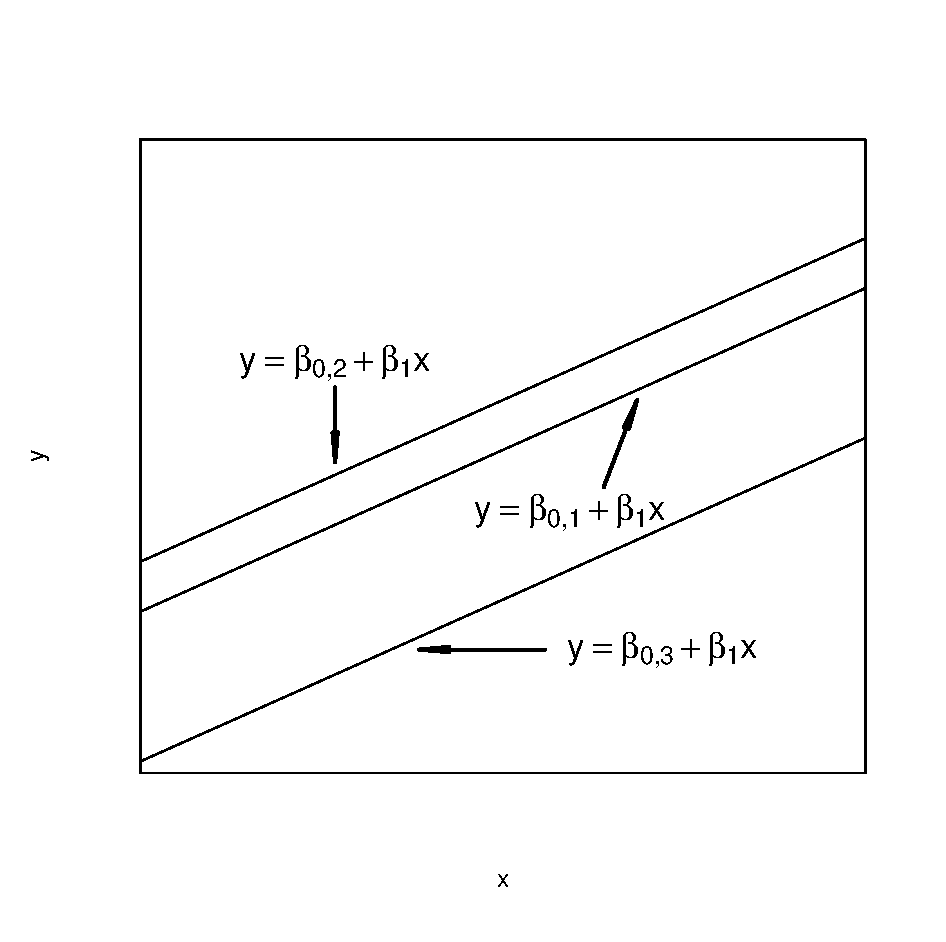
\includegraphics[width=1\textwidth,angle=0,scale=0.45]{Chapter4/Fig4_5A.ps}
    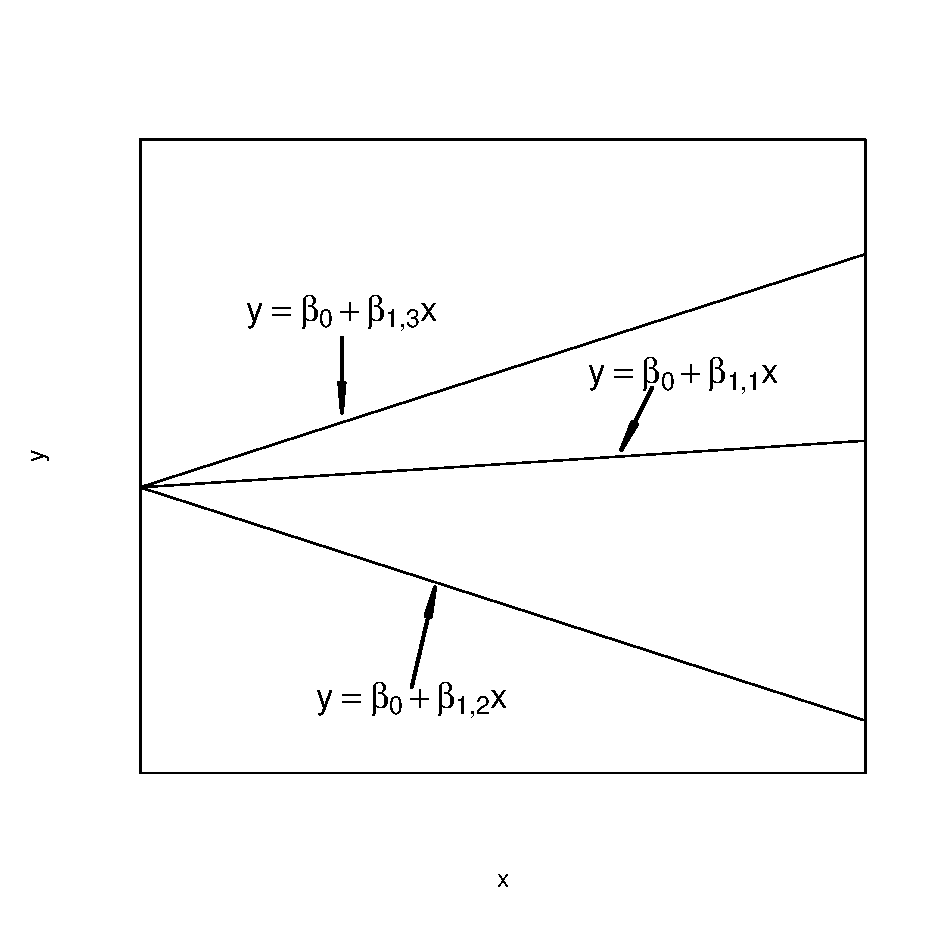
\includegraphics[width=1\textwidth,angle=0,scale=0.45]{Chapter4/Fig4_6A.ps} \hfill
     \parbox[t]{2.5in}{\caption{\label{F4:TheoryVarIntConSlope} \small  Plot of the expected response versus the covariate for the regression model
with variable intercept and constant slope.}} \hfill
    \parbox[t]{2.5in}{\caption{\label{F4:TheoryConIntVarSlope} \small  Plot of the expected response versus the covariate for the regression model
with constant intercept and variable slope.}}
  \end{center}
\end{figure}


\begin{figure}[htp]
  \begin{center}
    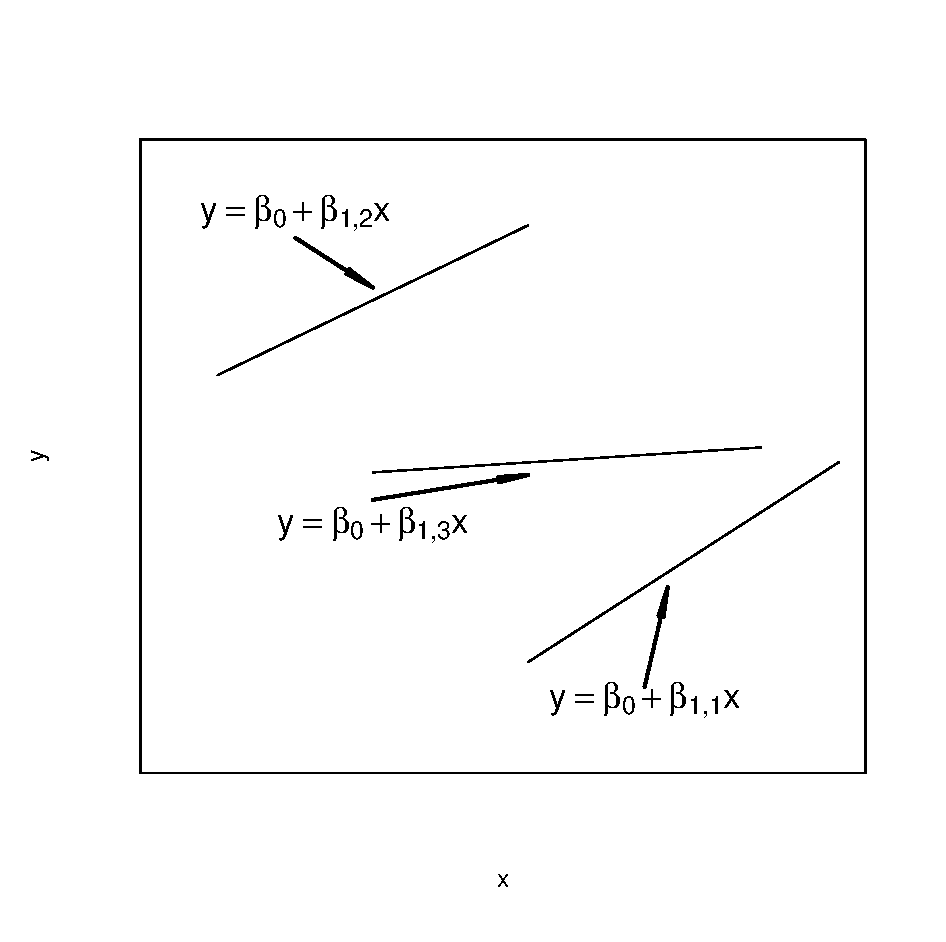
\includegraphics[width=1\textwidth,angle=0,scale=0.5]{Chapter4/Fig4_7A.ps}
    \caption{\label{F4:TheoryVarIntVarSlope} \small  Plot of the expected response versus the covariate for the regression model
with variable intercept and variable slope.}
  \end{center}
\end{figure}

For each model presented in Table \ref{T4:OneFactorCovariate},
parameter estimates can be calculated using the method of least
squares. As usual, this means writing the expected response, E
$y_{ij}$, as a function of known variables and unknown parameters.
Then, for candidate estimates of the parameters, an error sum of
squares can be calculated and minimized over all candidate
estimates. For the regression model with variable intercept and
constant slope, the least squares estimates can be expressed
compactly as:

\begin{equation*}
b_1=\frac{\sum_{j=1}^{c}\sum_{i=1}^{n_j}(x_{ij}-\bar{x}_j)(y_{ij}-\bar{%
y}_j)}{\sum_{j=1}^{c}\sum_{i=1}^{n_j}(x_{ij}-\bar{x}_j)^2}
\end{equation*}

\noindent and $b_{0,j}=\bar{y}_j-b_1\bar{x}_j$. Similarly, the least
squares estimates for the regression model with variable intercept
and slope can be expressed as:

\begin{equation*}
b_{1,j}=\frac{\sum_{i=1}^{n_j}(x_{ij}-\bar{x}_j)(y_{ij}-\bar{y}_j)}{%
\sum_{i=1}^{n_j}(x_{ij}-\bar{x}_j)^2}
\end{equation*}

\noindent and $b_{0,j}=\bar{y}_j-b_1\bar{x}_j$. With these parameter
estimates, fitted values may be calculated.

For each model, the error sum of squares is defined as the sum of
squared deviations between the observation and the corresponding
fitted values, that is,

\begin{equation*}
\text{Error
SS}=\sum_{j=1}^{c}\sum_{i=1}^{n_j}(y_{ij}-\hat{y}_{ij})^2.
\end{equation*}

\noindent Fitted values are defined to be the expected response with
the unknown parameters replaced by their least squares estimates.
For example, for the regression model with variable intercept and
constant slope the fitted values are
$\hat{y}_{ij}=b_{0,j}+b_1x_{ij}$.

\linejed


\empexjed{HospitalCosts}

\textbf{Example: Hospital Charges.}\ecaptionjed{Hospital Charges} We
now study the impact of various predictors on hospital charges in
the state of Wisconsin. Identifying predictors of hospital charges
can provide direction for hospitals, government, insurers and
consumers in controlling these factors that in turn leads to better
control of hospital costs. The data for the year 1989 were obtained
from the Office of Health Care Information, Wisconsin's Department
of Health and Human Services. Cross sectional data are used, which
details the 20 diagnosis related group (DRG) discharge costs for
hospitals in the state of Wisconsin, broken down into nine major
health service areas and three types of payer (Fee for service, HMO,
and other). Even though there are 540 potential DRG, area and payer
combinations $(20\times 9\times 3=540)$, only 526 combinations were
actually realized in the 1989 data set. Other predictor variables
included the logarithm of the total number of discharges (NO DSCHG)
and total number of hospital beds (NUM BEDS) for each combination.
The response variable is the logarithm of total hospital charges per
number of discharges (CHGNUM). To streamline the presentation, we
now consider only costs associated with three diagnostic related
groups (DRGs), DRG \#209, DRG \#391 and DRG \#430.

The covariate, $x$, is the natural logarithm of the number of
discharges. In ideal settings, hospitals with more patients enjoy
lower costs due to economies of scale. In non-ideal settings,
hospitals may not have excess capacity and thus, hospitals with more
patients have higher costs. One purpose of this analysis is to
investigate the relationship between hospital costs and hospital
utilization.

Recall that our measure of hospital charges is the logarithm of
costs per discharge $(y)$. The scatter plot in Figure
\ref{F4:CostperNumber} gives a preliminary idea of the relationship
between $y$ and $x$. We note that there appears to be a negative
relationship between $y$ and $x$.

The negative relationship between $y$ and $x$ suggested by Figure
\ref{F4:CostperNumber} is misleading and is induced by an
\textit{omitted variable}, the category of the cost (DRG). To see
the joint effect of the categorical variable DRG and the continuous
variable $x$, in Figure \ref{F4:DRGbyNumber} is a plot of $y$ versus
$x$ where the plotting symbols are codes for the level of the
categorical variable. From this plot, we see that the level of cost
varies by level of the factor DRG. Moreover, for each level of DRG,
the slope between $y$ and $x$ is either zero or positive. The slopes
are not negative, as suggested by Figure \ref{F4:CostperNumber}.

\begin{figure}[htp]
  \begin{center}
    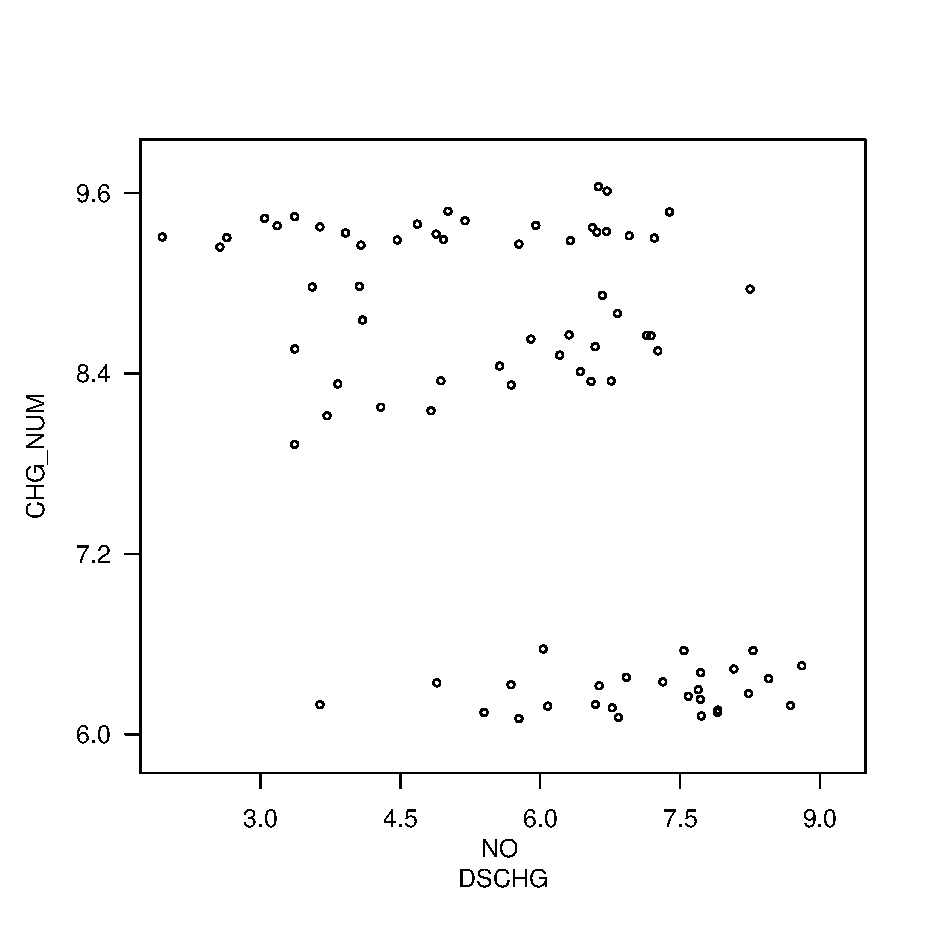
\includegraphics[width=1\textwidth,angle=0,scale=0.45]{Chapter4/Fig4_8A.ps}
    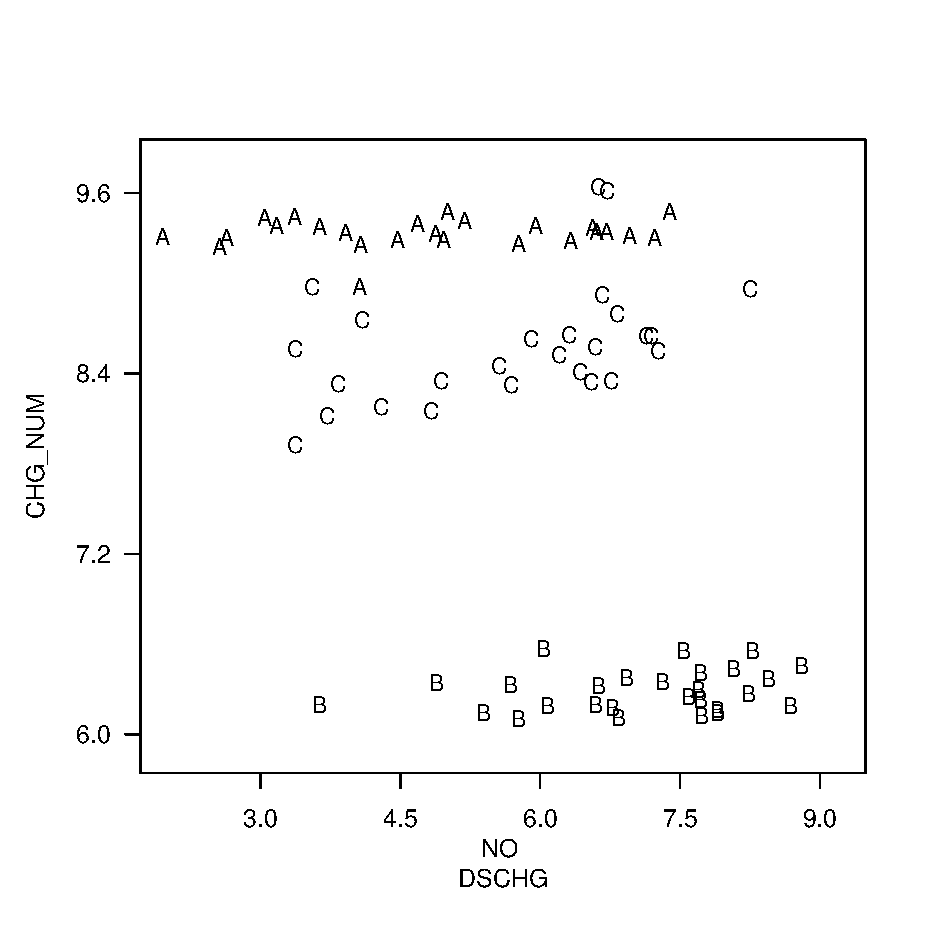
\includegraphics[width=1\textwidth,angle=0,scale=0.45]{Chapter4/Fig4_9A.ps} \hfill
    \parbox[t]{2.5in}{\caption{\label{F4:CostperNumber} \small  Plot of natural logarithm of cost per discharge versus natural
logarithm of the number of discharges.}} \hfill
    \parbox[t]{2.5in}{\caption{\label{F4:DRGbyNumber} \small  Letter plot of natural logarithm of cost per discharge versus natural
logarithm of the number of discharges by DRG. Here, A is for DRG
\#209, B is for DRG \#391 and C is for DRG \#430.}}
  \end{center}
\end{figure}


\begin{table}[h]
\caption{\label{T4:DRGModels} Degree of Freedom and Error Sum of
Squares of Several Models to Represent One Factor and One Covariate
for the DRG Example}
\begin{tabular}{lccrcc}
\hline & Model & Error & Error  &  & Error  \\
& degrees & degrees
& Sum & $R^2$  & Mean \\
Model Description & of freedom & of freedom & of Squares & (\%) &
Square
\\ \hline
One factor ANOVA & 2 &
76 & \multicolumn{1}{r}{$9.396$} & \multicolumn{1}{r}{$%
93.3$} & \multicolumn{1}{r}{$0.124$} \\
Regression with constant intercept & 1 & 77 &
\multicolumn{1}{r}{$115.059$} &
\multicolumn{1}{r}{$18.2$} & \multicolumn{1}{r}{$1.222$} \\
~~~and slope & & & & &  \\
Regression with variable intercept &3 & 75 &
\multicolumn{1}{r}{$7.482$} &
\multicolumn{1}{r}{$94.7$} & \multicolumn{1}{r}{$0.100$} \\
~~~and constant slope &  & &  &  &  \\
Regression with constant intercept & 3 & 75 &
\multicolumn{1}{r}{$14.048$} &
\multicolumn{1}{r}{$90.0$} & \multicolumn{1}{r}{$0.187$} \\
~~~and variable slope &  &  &  &  & \\
Regression with variable intercept & 5 & 73 &
\multicolumn{1}{r}{$5.458$} &
\multicolumn{1}{r}{$96.1$} & \multicolumn{1}{r}{$0.075$} \\
~~~and slope &  & & &  &  \\
\hline
\end{tabular}

\end{table}

Each of the five models defined in Table \ref{T4:OneFactorCovariate}
was fit to this subset of the Hospital case study. The summary
statistics are in Table \ref{T4:DRGModels}. For this data set, there
are $n=79$ observations and $c=3$ levels of the DRG factor. For each
model, the model degrees of freedom is the number of model
parameters minus one. The error degrees of freedom is the number of
observations minus the number of model parameters.

Using binary variables, each of the models in Table
\ref{T4:OneFactorCovariate} can be written in a regression format.
As we have seen in Section \ref{S4:SeveralCoeff}, when a model can
be written as a subset of another, larger model, we have formal
testing procedures available to decide which model is more
appropriate. To illustrate this testing procedure with our DRG
example, from Table \ref{T4:DRGModels} and the associated plots, it
seems clear that the DRG factor is important. Further, a $t$-test,
not presented here, shows that the covariate $x$ is important. Thus,
let's compare the full model E $y_{ij} = \beta_{0,j} + \beta_{1,j}x$
to the reduced model E $y_{ij}=\beta_{0,j}+\beta_1x$. In other
words, is there a different slope for each DRG?

Using the notation from Section \ref{S4:SeveralCoeff}, we call the
variable intercept and slope the full model. Under the null
hypothesis, $H_0: \beta_{1,1}=\beta_{1,2}=\beta_{1,3}$, we get the
variable intercept, constant slope model. Thus, using the $F$-ratio
in equation (\ref{E4:FratioErrSumSquares}), we have

\begin{equation*}
F\text{-ratio}=\frac{(Error~SS)_{reduced}-(Error~SS)_{full}}{ps_{full}^2}=\frac{{7.482-5.458}}{2(0.075)}=13.535.
\end{equation*}

\noindent The 95$th$ percentile from the $F$-distribution with
$df_1=p=2$ and $df_2=(df)_{full}=73$ is approximately 3.13. Thus,
this test leads us to reject the null hypothesis and declare the
alternative, the regression model with variable intercept and
variable slope, to be valid.

\linejed

\subsubsection*{General Linear Model}

In Section \ref{S4:BinaryVar}, we saw that we only use $c-1$
indicator variables to represent a categorical variable with $c$
levels. Similarly, in Section 4.3 we saw that the one factor ANOVA
model could be expressed as a regression model with $c$ indicator
variables. However, if we had attempted to estimate the model in
equation (\ref{E4:OneFactorTau}), the method of least squares would
not have arrived at a unique set of regression coefficient
estimates. The reason is that, in equation (\ref{E4:OneFactorTau}),
each explanatory variable can be expressed as a linear combination
of the others. For example, observe that $x_c = 1 - (x_1 + x_2 +
\ldots + x_{c-1})$.

The fact that parameter estimates are not unique is a drawback, but
not an overwhelming one. In fact, we now introduce the
\textit{general linear model},

\begin{equation} \label{E4:GeneralLinearModel}
y = \beta_0 + \beta_1 x_1 + \ldots \ + \beta_k x_k + \varepsilon,
\end{equation}

\noindent where $\{\varepsilon_i\}$ is a random sample from an
unknown population with mean zero. We follow standard terminology
and view the linear regression model as a special case of the
general linear model. To distinguish the two sets of models, we
assume that the explanatory variables are not linear combinations of
one another in the linear regression model context. This restriction
is not made in the general linear model case. To illustrate, the
models in equations (\ref{E4:OneFactorTau}) and (4.13) are examples
of general linear models that are not regression models.

In the linear regression model case, the assumption that the
explanatory variables are not linear combinations of one another
means that we can compute unique estimates of the regression
coefficients using the method of least squares. In the general
linear model case, the parameter estimates need not be unique.
However, an important feature of the general linear model is that
the resulting fitted values turn out to be unique, using the method
of least squares.

Specifically, suppose that we are considering the model in equation
(4.15) and, using the method of least squares, our regression
coefficient estimates are $b_0^{o}, b_1^{o}, \ldots, b_k^{o}$. This
set of regression coefficients estimates minimizes our error sum of
squares, but there are other sets of coefficients that also minimize
the error sum of squares. The fitted values are computed as
$\hat{y}_i = b_0^{o} + b_1^{o} x_{i1} + \ldots + b_k^{o} x_{ik}$. It
can be shown that the resulting fitted values are unique, in the
sense that any set of coefficients that minimize the error sum of
squares produce the same fitted values.

Thus, for a set of data and a specified general linear model, fitted
values are unique. Because residuals are computed as observed
responses minus fitted values, we have that the residuals are
unique. Because residuals are unique, we have the error sums of
squares are unique. Thus, it seems reasonable, and is true, that we
can use the general test of hypotheses described in Section
\ref{S4:SeveralCoeff} to decide whether collections of explanatory
variables are important.

To summarize, for general linear models, parameter estimates are not
unique and thus not meaningful. An important part of regression
models is the interpretation of regression coefficients. This
interpretation is not necessarily available in the general linear
model context. However, for general linear models, we may still
discuss the important of an individual variable or collection of
variables through partial \textit{F}-tests. Further, fitted values,
and the corresponding exercise of prediction, works in the general
linear model context. The advantage of the general linear model
context is that we need not worry about the type of restrictions to
impose on the parameters. Although not the subject of this text,
this advantage is particularly important in complicated experimental
designs used in the life sciences. Searle (1987) is one reference
for these designs and for further details of the general linear
model. The reader will find that general linear model estimation
routines are widely available in statistical software packages
available on the market today.



\section{Further Reading and References}


\textbf{Chapter References}

\begin{multicols}{2}

\scalefont{0.9}

Keeler, Emmett B., and  John E. Rolph (1988). The demand for
episodes of treatment in the Health Insurance Experiment.
\emph{Journal of Health Economics} 7: 337-367.

Searle, Shayle R. (1987). \textit{Linear Models for Unbalanced
Data}. John Wiley \& Sons, New York.


\scalefont{1.1111}

\end{multicols}

\bigskip


\section{Exercises}

\scalefont{0.90}

\begin{exercises}

\item In this exercise, we consider relating two statistics that summarize how well a regression model fits,
the $F$-ratio and $R^2$, the coefficient of determination. (Here,
the $F$-ratio is the statistic used to test model adequacy, not a
partial $F$ statistic.)

a.  Write down both $R^2$ in terms of Error SS and Regression SS.

b. Write down $F$-ratio in terms of Error SS, Regression SS , $k$
and $n$.

c. Establish the algebraic relationship
\begin{equation*}
F-\textrm{ratio} = \frac{R^2}{1-R^2} \frac{n-(k+1)}{k}.
\end{equation*}

d.  Suppose that $n = 40$, $k = 5$ and $R^2 = 0.20$. Calculate the
$F$-ratio. Perform the usual test of model adequacy to determine
whether or not the five explanatory variables jointly significantly
affect the response variable.

e.  Suppose that $n = 400$ (not 40), $k = 5$ and $R^2 = 0.20$.
Calculate the $F$-ratio. Perform the usual test of model adequacy to
determine whether or not the five explanatory variables jointly
significantly affect the response variable.

\empexjed{HCUPSample}

\item \textbf{Hospital expenditures.}\label{Ex:HospExpend4} This exercise considers
hospital expenditures data provided by the US Agency for Healthcare
Research and Quality (AHRQ) and described in Exercise
1.\ref{Ex:HospExpend}.

a. Produce a scatter plot, correlation and a linear regression of
LNTOTCHG on AGE. Is AGE a significant predictor of LNTOTCHG?

b. You are concerned that newborns follow a different pattern than
other ages. Create a binary variable that indicates whether or not
AGE equals zero. Run a regression using this binary variable and AGE
as explanatory variables. It is the binary variable statistically
significant?

c. Now examine the gender effect, using the binary variable FEMALE
that is one if the patient is female and zero otherwise. Run a
regression using AGE and FEMALE as explanatory variables. Run a
second regression running these two variables with an interaction
term. Comment on whether the gender effect is important in either
model.

d. Now consider the type of admission, APRDRG, an acronym for ``all
patient refined diagnostic related group.'' This is a categorical
explanatory variable that provides information on the type of
hospital admission. There are several hundred levels of this
category. For example, level 640 represents admission for a normal
newborn, with neonatal weight greater than or equal to 2.5
kilograms. As another example, level 225 represents admission
resulting in an appendectomy.

e(i). Run a one-factor ANOVA model, using APRDRG to predict
LNTOTCHG. Examine the $R^2$ and the coefficient of determination of
the linear regression model of LNTOTCHG on AGE. Based on this
comparison, which model do you think is preferred?

e(ii). For the one-factor model in part f(i), provide a 95\%
confidence interval for LNTOTCHG for level 225 corresponding to an
appendectomy. Convert your final anwer from logarithmic dollars to
dollars via exponentiation.

e(iii). Run a regression model of APRDRG, FEMALE and AGE on
LNTOTCHG. State whether AGE is a statistically significant predictor
of LNTOTCHG. State whether FEMALE is a statistically significant
predictor of LNTOTCHG.

\empexjed{WiscNursingHome}

\item \textbf{Nursing home utilization.}\label{Ex:NursHome4} This exercise considers nursing
home data provided by the Wisconsin Department of Health and Family
Services (DHFS) and described in Exercises 1.\ref{Ex:NursHome},
2.\ref{Ex:NursHome2a} and 2.\ref{Ex:NursHome2b}.

In addition to the size variables, we also have information on
several binary variables. The variable URBAN is used to indicate the
facility's location. It is one if the facility is located in an
urban environment and zero otherwise. The variable MCERT indicates
whether the facility is Medicare-certified. Most, but not all,
nursing homes are certified to provide Medicare-funded care. There
are three organizational structures for nursing homes. They are
government (state, counties, municipalities), for-profit businesses,
and tax-exempt organizations. Periodically, facilities may change
ownership and, less frequently, ownership type. We create two binary
variables PRO and TAXEXEMPT to denote for-profit business and
tax-exempt organizations, respectively. Some nursing homes opt not
to purchase private insurance coverage for their employees. Instead,
these facilities directly provide insurance and pension benefits to
their employees; this is referred to as ``self funding of
insurance." We use binary variable SELFFUNDINS to denote it.

You decide to examine the relationship between LOGTPY(y) and the
explanatory variables. Use cost report year 2001 data, and do the
following analysis.

a. There are three levels of organizational structures, but we only
use two binary variables (PRO and TAXEXEMPT). Explain why.

b. Run a one-way analysis of variance using TAXEXEMPT as the factor.
Decide whether or not tax-exempt is an important factor in
determining LOGTPY. State your null hypothesis, alternative
hypothesis and all components of the decision-making rule. Use a 5\%
level of significance.

c. Run a one-way analysis of variance using MCert as the factor.
Decide whether or not location is an important factor in determining
LOGTPY.

c(i). Provide a point estimate of LOGTPY for a nursing facility that
is not Medicare-Certified.

c(ii).  Provide a 95\% confidence interval for your point estimate
in part (i).

d. Run a regression model using the binary variables, URBAN, PRO,
TAXEXEMPT, SELFFUNDINS, and MCERT. Find $R^2$. Which variables are
statistically significant?

e. Run a regression model using all explanatory variables,
LOGNUMBED, LOGSQRFOOT, URBAN, PRO, TAXEXEMPT, SELFFUNDINS, and
MCERT. Find $R^2$. Which variables are statistically significant?

e(i). Calculate the partial correlation between LOGTPY and
LOGSQRFOOT. Compare this to the correlation between LOGTPY and
LOGSQRFOOT. Explain why the partial correlation is small.

e(ii). Compare the low level of the $t$-ratios (for testing the
importance of individual regression coefficients) and the level of
the $F$-ratio (for testing model adequacy). Describing the seeming
inconsistency, and provide an explanation for this inconsistency.

\empexjed{AutoClaims}

\item \textbf{Automobile insurance claims.}\label{Ex:AutoClaims4} Refer to Exercise
1.\ref{Ex:AutoClaims}.

a. Run a regression of LNPAID on AGE. Is AGE a statistically
significant variable? To respond to this question, use a formal test
of hypothesis. State your null and alternative hypotheses,
decision-making criterion, and your decision-making rule. Also
comment on the goodness of fit of this variable.

b. Consider using class as a single explanatory variable. Use the
one factor to estimate the model and respond to the following
questions.

b(i). What is the point estimate of claims in class C7, drivers
50-69, driving to work or school, less than 30 miles per week with
annual mileage under 7500, in natural logarithmic units?

b(ii). Determine the corresponding 95\% confidence interval of
expected claims, in natural logarithmic units.

b(iii). Convert the 95\% confidence interval of expected claims that
you determined in part b(ii) to dollars.

c. Run a regression of LNPAID on AGE, GENDER and the categorical
variables STATE CODE and CLASS.

c(i). Is GENDER a statistically significant variable? To respond to
this question, use a formal test of hypothesis. State your null and
alternative hypotheses, decision-making criterion, and your
decision-making rule.

c(ii). Is CLASS a statistically significant variable? To respond to
this question, use a formal test of hypothesis. State your null and
alternative hypotheses, decision-making criterion, and your
decision-making rule.

c(iii). Use the model to provide a point estimate of claims in
dollars (not log dollars) for a male in STATE 2 in CLASS C7.

c(iv). Write down the coefficient associated with CLASS C7 and
interpret this coefficient.

\empexjed{WiscLottery}

\item \textbf{Wisconsin lottery.}\label{Ex:Lottery4}
This exercise considers State of Wisconsin lottery sales data that
were described in Section 2.1 and examined in Exercise
3.\ref{Ex:Lottery3}.

\textbf{Part 1:} You decide to examine the relationship between
SALES ($y$) and all eight explanatory variables (PERPERHH, MEDSCHYR,
MEDHVL, PRCRENT, PRC55P, \newline HHMEDAGE, MEDINC, and POP).

a. Fit a regression model of OLSALES on all eight explanatory
variables.

b. Find $R^2$.

b(i). Use it to calculate the correlation coefficient between the
observed and fitted values.

b(ii). You want to use $R^2$ to test the adequacy of the model in
part (a). Use a formal test of hypothesis. State your null and
alternative hypothesis, decision-making criterion, and your
decision-making rules.

c. Test whether POP, MEDSCHYR and MEDHVL are jointly important
explanatory variables for understanding OLSALES.


\textbf{Part 2:} After the preliminary analysis in Part 1, you
decide to examine the relationship between SALES($y$) and POP,
MEDSCHYR, and MEDHVL.

a. Fit a regression model of OLSALES on these three explanatory
variables.

b. Has the coefficient of determination decreased from the eight
variable regression model to the three variable model? Does this
mean that the model is not improved or does it provide little
information? Explain your response.

c. To state formally whether one should use the three or eight
variable model, use a partial $F$-test. State your null and
alternative hypotheses, decision-making criterion, and your
decision-making rules.

\empexjed{NAICExpense}

\item \textbf{Insurance company expenses.}\label{Ex:NAICExpense4}
This exercise considers insurance company data from the NAIC and
described in Exercises 1.\ref{Ex:NAICExpense} and
3.\ref{Ex:NAICExpense3}.


a. Are the quadratic terms important?

Consider a linear model of LNEXPENSES on twelve explanatory
variables. For the explanatory variables, include assets, GROUP,
both versions of losses and gross premiums, as well as the two BLS
variables. Also include the square each of the two loss and the two
gross premium variables.

Test whether the four squared terms are jointly statistically
significant, using a partial $F$-test. State your null and
alternative hypotheses, decision-making criterion, and your
decision-making rules.

b. Are the interaction terms with GROUP important?

Omit the two BLS variables, so that now there are eleven variables,
assets, GROUP, both versions of losses and gross premiums, as well
as interactions of GROUP with assets and both versions of losses and
gross premiums.

Test whether the five interaction terms are jointly statistically
significant, using a partial $F$-test. State your null and
alternative hypotheses, decision-making criterion, and your
decision-making rules.

c. You are examining a company that is not in the sample with values
LOSSLONG = 25, LOSSSHORT = 40, GPWPERSONAL= 50, GPWCOMM= 120, ASSETS
= 400,CASH= 350, and GROUP = 1.

Use the eleven variable interaction model in part (b) to produce a
95\% prediction interval for this company.

\empexjed{UNLifeExpectancy}

\item \textbf{National Life Expectancies.}\label{Ex:UNLIFE4} We
continue the analysis begun in Exercises 1.\ref{Ex:UNLIFE},
2.\ref{Ex:UNLIFE2} and 3.\ref{Ex:UNLIFE3}.

a. Consider the regression using three explanatory variables,
FERTILITY, PUBLICEDUCATION and lnHEALTH that you did in Exercise
3.\ref{Ex:UNLIFE3}. Test whether PUBLICEDUCATION and lnHEALTH are
jointly statistically significant, using a partial $F$-test. State
your null and alternative hypotheses, decision-making criterion, and
your decision-making rules. (Hint: Use the coefficient of
determination form for calculating the test statistic.) Provide an
approximate $p$-value for the test.

b. We now introduce the REGION variable, summarized in Table
\ref{Ex:UNLIFERegionStats}. A boxplot of life expectancies versus
REGION is given in Figure \ref{Ex:UNLIFEPlot3}. Describe what we
learn from the Table and boxplot about the effect of REGION on
LIFEEXP.


\begin{figure}[htp]
  \begin{center}
   \includegraphics[width=1\textwidth,angle=270,scale=0.25]{Exercises/UNLIFEPlot3.ps}
   \caption{\label{Ex:UNLIFEPlot3} \small  Boxplots of LIFEEXP by REGION.}
  \end{center}
\end{figure}


\begin{table}[h]

\scalefont{0.8} \caption{\label{Ex:UNLIFERegionStats} \small Average
Life Expectancy by Region}
\begin{center}
\begin{tabular}{c|lcr}
\hline
    REGION & Region Description &     Number &       Mean \\ \hline
         1 & Arab States &         13 &       71.9 \\
         2 & East Asia and the Pacific &         17 &       69.1 \\
         3 & Latin American and the Carribean &         25 &       72.8 \\
         4 & South Asia &          7 &       65.1 \\
         5 & Southern Europe &          3 &       67.4 \\
         6 & Sub-Saharan Africa &         38 &       52.2 \\
         7 & Central and Eastern Europe &         24 &       71.6 \\
         8 & High Income OECD &         23 &       79.6 \\\hline
           & All          &        150 &     67.4       \\\hline
\end{tabular}
\end{center}\scalefont{1.25}
\end{table}

c. Fit a regression model using only the factor, REGION. Is REGION a
statistically significant determinant of LIFEEXP? State your null
and alternative hypotheses, decision-making criterion, and your
decision-making rules.

d. Fit a regression model using three explanatory variables,
FERTILITY, PUBLICEDUCATION and lnHEALTH, as well as the categorical
variable REGION.

d(i). You are examining a country is not in the sample with values
FERTILITY= 2.0, PUBLICEDUCATION= 5.0,  and lnHEALTH= 1.0. Produce
two predicted life expectancy values by assuming that the country is
from (1) an Arab state and (2) Sub-Sahara Africa.

d(ii). Provide a 95\% confidence interval for the difference in life
expectancies between an Arab state and a country from Sub-Sahara
Africa.

d(iii). Provide the (usual ordinary least squares) point estimate
for the difference in life expectancies between a country from
Sub-Sahara Africa and a high income OECD (Organization for Economic
Co-operation and Development) country.

\end{exercises}
\scalefont{1.1111}

\section{Technical Supplement - Matrix Expressions}
 \setcounter{equation}{12}
\subsection{Expressing Models with Categorical Variables in
Matrix Form}\label{S4:CatVarMatrix}

Chapter 3 showed how to write the regression model equation in the
form $\mathbf{y=X} \boldsymbol \beta + \boldsymbol \varepsilon$
where $\mathbf{X}$ is a matrix of explanatory variables. This form
permits straightforward calculation of regression coefficients,
$\mathbf{b} = \left(\mathbf{X}^{\prime}
\mathbf{X}\right)^{-1}\mathbf{X}^{\prime} \mathbf{y}$. This section
shows how the model and calculations reduce to simpler expressions
when the explanatory variables are categorical.


\textbf{One Categorical Variable Model.} Consider the model with one
categorical variable introduced in Section \ref{S4:OneFactor} with
$c$ levels of the categorical variable. From equations
(\ref{E4:OneFactorEquation}) and (\ref{E4:OneFactor}), this model
can be written as
\begin{equation*}
y_{ij} = \mu_1 z_{i1} + \mu_2 z_{i2} + \ldots + \mu_c z_{ic} +
\varepsilon_{ij}.
\end{equation*}
Here, $z_{ij}$ is a variable that indicates whether the observation
falls in the $j$th categorical level. This can be expressed as

\begin{equation}\label{E4:MatrixOneFactor}
\mathbf{y}=
\begin{bmatrix}
y_{1,1} \\
\cdot  \\
\cdot  \\
\cdot  \\
y_{n_1,1} \\
\cdot  \\
\cdot  \\
\cdot  \\
y_{1,c} \\
\cdot  \\
\cdot  \\
\cdot  \\
y_{n_{c},c}%
\end{bmatrix}
=
\begin{bmatrix}
1 & 0 & \cdot \cdot \cdot  & 0 \\
\cdot  & \cdot  & \cdot \cdot \cdot  & \cdot  \\
\cdot  & \cdot  & \cdot \cdot \cdot  & \cdot  \\
\cdot  & \cdot  & \cdot \cdot \cdot  & \cdot  \\
1 & 0 & \cdot \cdot \cdot  & \cdot  \\
\cdot  & \cdot  & \cdot \cdot \cdot  & \cdot  \\
\cdot  & \cdot  & \cdot \cdot \cdot  & \cdot  \\
\cdot  & \cdot  & \cdot \cdot \cdot  & \cdot  \\
0 & 0 & \cdot \cdot \cdot  & 1 \\
\cdot  & \cdot  & \cdot \cdot \cdot  & \cdot  \\
\cdot  & \cdot  & \cdot \cdot \cdot  & \cdot  \\
\cdot  & \cdot  & \cdot \cdot \cdot  & \cdot  \\
0 & 0 & \cdot \cdot \cdot  & 1%
\end{bmatrix}%
\begin{bmatrix}
\mu_1 \\
\cdot  \\
\cdot  \\
\cdot  \\
\mu_c
\end{bmatrix}
+
\begin{bmatrix}
\varepsilon_{1,1} \\
\cdot  \\
\cdot  \\
\cdot  \\
\varepsilon_{n_1,1} \\
\cdot  \\
\cdot  \\
\cdot  \\
\varepsilon_{1,c} \\
\cdot  \\
\cdot  \\
\cdot  \\
\varepsilon_{n_{c},c}
\end{bmatrix}
=\mathbf{X} \boldsymbol \beta + \boldsymbol \varepsilon .
\end{equation}
To make the notation more compact, we write $\mathbf{0}$ and
$\mathbf{1}$ for a column of zeros and ones, respectively. With this
convention, another way to express equation
(\ref{E4:MatrixOneFactor}) is

\begin{center}
\begin{equation}\label{E4:Matrix2OneFactor}
\mathbf{y}=%
\begin{bmatrix}
\mathbf{1}_1 & \mathbf{0}_1 & \cdot \cdot \cdot  & \mathbf{0}%
_1 \\
\mathbf{0}_2 & \mathbf{1}_2 & \cdot \cdot \cdot  & \mathbf{0}%
_2 \\
\cdot  & \cdot  & \cdot \cdot \cdot  & \cdot  \\
\cdot  & \cdot  & \cdot \cdot \cdot  & \cdot  \\
\cdot  & \cdot  & \cdot \cdot \cdot  & \cdot  \\
\mathbf{0}_c & \mathbf{0}_c & \cdot \cdot \cdot  & \mathbf{1}_c
\end{bmatrix}
\begin{bmatrix}
\mu_1 \\
\mu_2 \\
\cdot  \\
\cdot  \\
\cdot  \\
\mu_c%
\end{bmatrix}
+\boldsymbol \varepsilon = \mathbf{X} \boldsymbol \beta +
\boldsymbol \varepsilon .
\end{equation}
\end{center}

\noindent Here, $\mathbf{0}_1$ and $\mathbf{1}_1$ stand for vector
columns of length $n_1$ of zeros and ones, respectively, and
similarly for $\mathbf{0}_2, \mathbf{1}_2, \ldots, \mathbf{0}_c,
\mathbf{1}_c$.

Equation (\ref{E4:Matrix2OneFactor}) allows us to apply the
machinery developed for the regression model to the model with one
categorical variable. As an intermediate calculation, we have

\begin{center}
\begin{eqnarray}\label{E4:OneFactorXPrimeX}
(\mathbf{X^{\prime}X})^{-1} &=&\left(
\begin{bmatrix}
\mathbf{1}_1 & \mathbf{0}_2 & \cdot \cdot \cdot  & \mathbf{0}_c \\
\mathbf{0}_1 & \mathbf{1}_2 & \cdot \cdot \cdot  & \mathbf{0}_c \\
\cdot  & \cdot  & \cdot \cdot \cdot  & \cdot  \\
\cdot  & \cdot  & \cdot \cdot \cdot  & \cdot  \\
\cdot  & \cdot  & \cdot \cdot \cdot  & \cdot  \\
\mathbf{0}_1 & \mathbf{0}_2 & \cdot \cdot \cdot  & \mathbf{1}_c%
\end{bmatrix}^{\prime}%
\begin{bmatrix}
\mathbf{1}_1 & \mathbf{0}_1 & \cdot \cdot \cdot  & \mathbf{0}%
_1 \\
\mathbf{0}_2 & \mathbf{1}_2 & \cdot \cdot \cdot  & \mathbf{0}%
_2 \\
\cdot  & \cdot  & \cdot \cdot \cdot  & \cdot  \\
\cdot  & \cdot  & \cdot \cdot \cdot  & \cdot  \\
\cdot  & \cdot  & \cdot \cdot \cdot  & \cdot  \\
\mathbf{0}_{c} & \mathbf{0}_{c} & \cdot \cdot \cdot  & \mathbf{1}_c
\end{bmatrix} \notag
\right) ^{-1} \\
&=&%
\begin{bmatrix}
n_1 & 0 & \cdot \cdot \cdot  & 0 \\
0 & n_2 & \cdot \cdot \cdot  & 0 \\
\cdot  & \cdot  & \cdot \cdot \cdot  & \cdot  \\
\cdot  & \cdot  & \cdot \cdot \cdot  & \cdot  \\
\cdot  & \cdot  & \cdot \cdot \cdot  & \cdot  \\
0 & 0 & \cdot \cdot \cdot  & n_c%
\end{bmatrix}%
^{-1}=%
\begin{bmatrix}
\frac{1}{n_1} & 0 & \cdot \cdot \cdot  & 0 \\
0 & \frac{1}{n_2} & \cdot \cdot \cdot  & 0 \\
\cdot  & \cdot  & \cdot \cdot \cdot  & \cdot  \\
\cdot  & \cdot  & \cdot \cdot \cdot  & \cdot  \\
\cdot  & \cdot  & \cdot \cdot \cdot  & \cdot  \\
0 & 0 & \cdot \cdot \cdot  & \frac{1}{n_c}
\end{bmatrix}%
.
\end{eqnarray}
\end{center}

Thus, the parameter estimates are

\begin{center}
\begin{eqnarray}\label{E4:OneFactorXPrimeXinvXPrimey}
\mathbf{b} &=&%
\begin{bmatrix}
\hat{\mu}_1 \\
\cdot  \\
\cdot  \\
\cdot  \\
\hat{\mu}_{c}%
\end{bmatrix}%
=\mathbf{(X}^{\prime}\mathbf{X)}^{-1}\mathbf{X}^{\prime}\mathbf{y}=%
\begin{bmatrix}
\frac{1}{n_1} & 0 & \cdot \cdot \cdot  & 0 \\
0 & \frac{1}{n_2} & \cdot \cdot \cdot  & 0 \\
\cdot  & \cdot  & \cdot \cdot \cdot  & \cdot  \\
\cdot  & \cdot  & \cdot \cdot \cdot  & \cdot  \\
\cdot  & \cdot  & \cdot \cdot \cdot  & \cdot  \\
0 & 0 & \cdot \cdot \cdot  & \frac{1}{n_c}
\end{bmatrix}
\begin{bmatrix}
\mathbf{1}_1 & \mathbf{0}_2 & \cdot \cdot \cdot  & \mathbf{0}_c \\
\mathbf{0}_1 & \mathbf{1}_2 & \cdot \cdot \cdot  & \mathbf{0}_c \\
\cdot  & \cdot  & \cdot \cdot \cdot  & \cdot  \\
\cdot  & \cdot  & \cdot \cdot \cdot  & \cdot  \\
\cdot  & \cdot  & \cdot \cdot \cdot  & \cdot  \\
\mathbf{0}_1 & \mathbf{0}_2 & \cdot \cdot \cdot  & \mathbf{1}_c%
\end{bmatrix} ^{\prime}
\begin{bmatrix}
y_{1,1} \\
\cdot  \\
\cdot  \\
\cdot  \\
y_{n_1,1} \\
\cdot  \\
\cdot  \\
\cdot  \\
y_{1,c} \\
\cdot  \\
\cdot  \\
\cdot  \\
y_{n_{c},c}%
\end{bmatrix} \notag
\\
&=&%
\begin{bmatrix}
\frac{1}{n_1} & 0 & \cdot \cdot \cdot  & 0 \\
0 & \frac{1}{n_2} & \cdot \cdot \cdot  & 0 \\
\cdot  & \cdot  & \cdot \cdot \cdot  & \cdot  \\
\cdot  & \cdot  & \cdot \cdot \cdot  & \cdot  \\
\cdot  & \cdot  & \cdot \cdot \cdot  & \cdot  \\
0 & 0 & \cdot \cdot \cdot  & \frac{1}{n_c}
\end{bmatrix}
\begin{bmatrix}
\sum_{i=1}^{n_1}y_{i1} \\
\cdot  \\
\cdot  \\
\cdot  \\
\sum_{i=1}^{n_{c}}y_{ic}%
\end{bmatrix}%
=%
\begin{bmatrix}
\bar{y}_1 \\
\cdot  \\
\cdot  \\
\cdot  \\
\bar{y}_c
\end{bmatrix} .
\end{eqnarray}
\end{center}

We have seen that the least squares estimate of $\mu_j$,
$\bar{y}_j$, can been obtained directly from equation
(\ref{E4:OneFactor}). By rewriting the model in matrix regression
notation, we can appeal to linear regression model results and need
not prove properties of models with categorical variables from first
principles. That is, because this model is in regression format, we
immediately have all the properties of the regression model.

Telling your software package that a variable is categorical can
mean more efficient calculations, as in the calculations of the least
square regression estimates in equation (\ref{E4:OneFactorXPrimeXinvXPrimey}).
Further, calculation of other quantities can also be done more directly.
As another example, we have that the standard
error of $\hat{\mu}_j$ is

\begin{equation*}
se(\hat{\mu}_j) = s ~ \sqrt{j\text{th \textit{diagonal element} of }
\mathbf{(X}^{\prime}\mathbf{X)}^{-1}} = s/\sqrt{n_j}.
\end{equation*}

\textbf{One Categorical and One Continuous Variable Model.} As
another illustration, we consider the variable intercept and
constant slope model in Table \ref{T4:OneFactorCovariate}. This can
be expressed as a regression model using binary variables as

\begin{center}
\[
y_{ij}=\beta_{01}z_{i1}+\beta_{02}z_{i2}+\ldots+\beta
_{0c}z_{ic}+\beta_1x_{ij}+\varepsilon_{ij}.
\]
\end{center}

\noindent Here, $z_{ij}$ is an indicator variable that the observation falls in the $j$%
th level. This can be expressed as $\mathbf{y}=%
\mathbf{X \boldsymbol \beta + \boldsymbol \varepsilon}$ where

\begin{equation}\label{E4:CategoricalContinuous}
\mathbf{X}=%
\begin{bmatrix}
\mathbf{1}_1 & \mathbf{0}_1 & \cdot \cdot \cdot  & \mathbf{0}%
_1 & \mathbf{x}_1 \\
\mathbf{0}_2 & \mathbf{1}_2 & \cdot \cdot \cdot  & \mathbf{0}%
_2 & \mathbf{x}_2 \\
\cdot  & \cdot  & \cdot \cdot \cdot  & \cdot  & \cdot  \\
\cdot  & \cdot  & \cdot \cdot \cdot  & \cdot  & \cdot  \\
\cdot  & \cdot  & \cdot \cdot \cdot  & \cdot  & \cdot  \\
\mathbf{0}_{c} & \mathbf{0}_{c} & \cdot \cdot \cdot  & \mathbf{1}_c & \mathbf{x}_{c}%
\end{bmatrix}%
\text{ \ \ \ \ and \ \ \ }\boldsymbol \beta=
\begin{bmatrix}
\beta_{01} \\
\beta_{02} \\
\cdot  \\
\cdot  \\
\cdot  \\
\beta_{0c} \\
\beta_1%
\end{bmatrix}
\end{equation}

\noindent As before, $\mathbf{0}_j$ and $\mathbf{1}_j$ stand for
vector columns of length $n_j$ of zeros and ones, respectively.
Further, $\mathbf{x}_j=(x_{1j},x_{2j},\ldots,x_{n_j,j})^{\prime}$ is
the column of the continuous variable at the $j$th level. Now,
straight-forward matrix algebra techniques provide the least squares
estimates.

\subsection{Calculating Least Squares Estimates Successively}\label{S4:MatrixSuccess}

When computing regression coefficients using least squares,
$\mathbf{b} = \left( \mathbf{X}^{\prime}\mathbf{X}\right)^{-1}
\mathbf{X}^{\prime}\mathbf{y}$, for some applications, the dimension
of $\mathbf{X}^{\prime}\mathbf{X}$ can be large, causing
computational difficulties. Fortunately, for some problems, the
computations can be partitioned into smaller problems that can be
solved in succession.

\boxedjed
\emph{Successive Least Squares Calculation.} Suppose that the regression function can be written as
\begin{equation*}
\mathrm{E}~\mathbf{y} = \mathbf{X} \boldsymbol \beta = \left(
\mathbf{X}_1 : \mathbf{X}_2 \right) \left(
\begin{array}{c}
\boldsymbol \beta_1  \\
\boldsymbol \beta_2  \\
\end{array}
\right) ,
\end{equation*}
where $\mathbf{X}_1$ has dimensions $n \times k_1$, $\mathbf{X}_2$
has dimensions $n \times k_2$, $k_1+k_2=k$, $\boldsymbol \beta_1 $
has dimensions $k_1 \times 1$ and $\boldsymbol \beta_2 $ has
dimensions $k_2 \times 1$. Define $\mathbf{Q}_1 = \mathbf{I} - \mathbf{X}_1
\left(\mathbf{X}_1^{\prime}\mathbf{X}_1 \right)^{-1}
\mathbf{X}_1^{\prime}.$ Then, the least squares estimator can be computed as:

\begin{equation}\label{E4:PartitionOLS}
\mathbf{b} = \left(
  \begin{array}{c}
    \mathbf{b}_1\\
    \mathbf{b}_2\\
  \end{array}
\right)
=
\left(
  \begin{array}{c}
    (\mathbf{X}_1^{\prime}\mathbf{X}_1)^{-1}\mathbf{X}_1^{\prime}
\left(
\mathbf{y} - \mathbf{X}_2 \mathbf{b}_2
\right)\\
   \left(\mathbf{X}_2^{\prime} \mathbf{Q}_1 \mathbf{X}_2
\right)^{-1} \mathbf{X}_2^{\prime} \mathbf{Q}_1\mathbf{y}\\
  \end{array}
\right)
\end{equation}

\end{boxedminipage}
\bigskip

\linejed

\textbf{Special Case: One Categorical and One Continuous Variable Model}.
To illustrate the relevance of equation (\ref{E4:PartitionOLS}), let us return to
the model summarized in equation (\ref{E4:CategoricalContinuous}). Here,
we saw that the dimension of $\mathbf{X}$ is $n \times (c+1)$ and so the dimension of
$\mathbf{X}^{\prime}\mathbf{X}$ is $(c+1) \times (c+1)$. Taking the inverse of this
matrix could be difficult if $c$ is large, say in the thousands. To apply equation
(\ref{E4:PartitionOLS}), we define
\begin{equation*}
\mathbf{X}_1=
\begin{bmatrix}
\mathbf{1}_1 & \mathbf{0}_1 & \cdot \cdot \cdot  & \mathbf{0}
_1 \\
\mathbf{0}_2 & \mathbf{1}_2 & \cdot \cdot \cdot  & \mathbf{0}
_2 \\
\cdot  & \cdot  & \cdot \cdot \cdot  & \cdot  \\
\cdot  & \cdot  & \cdot \cdot \cdot  & \cdot  \\
\cdot  & \cdot  & \cdot \cdot \cdot  & \cdot  \\
\mathbf{0}_{c} & \mathbf{0}_{c} & \cdot \cdot \cdot  & \mathbf{1}_c
\end{bmatrix}
\text{ \ \ \ \ and \ \ \ }\mathbf{X}_2 =
\begin{bmatrix}
\mathbf{x}_1\\
\mathbf{x}_2 \\
\cdot  \\
\cdot  \\
\cdot  \\
\mathbf{x}_c \\
\end{bmatrix} .
\end{equation*}
In this case, we have seen in equation (\ref{E4:OneFactorXPrimeX}) how it
is straightforward to compute
$\left(\mathbf{X}_1^{\prime}\mathbf{X}_1 \right)^{-1}$ without requiring
matrix inversion. This means that calculating $\mathbf{Q}_1$ is also straightforward. With this,
we can compute $\mathbf{X}_2^{\prime} \mathbf{Q}_1 \mathbf{X}_2$ and, because it is a scalar,
immediately get its inverse. This gives us $\mathbf{b}_2$ and then we use this result to
calculate $\mathbf{b}_1$. Although this procedure is not as direct as the our usual expression
$\mathbf{b} = \left( \mathbf{X}^{\prime}\mathbf{X}\right)^{-1}
\mathbf{X}^{\prime}\mathbf{y}$, it can be much more computationally efficient.

\linejed

To establish equation (\ref{E4:PartitionOLS}),
we use two results that are standard matrix algebra results on
inverses of partitioned matrices.

\textbf{Partitioned Matrix Results.} Suppose that we can partition
the $(p+q)\times (p+q)$ matrix $\mathbf{B}$ as
\begin{equation*}
\mathbf{B}=%
\begin{bmatrix}
\mathbf{B}_{11} & \mathbf{B}_{12} \\
\mathbf{B}_{12}^{\prime } & \mathbf{B}_{22}%
\end{bmatrix},
\end{equation*}
where $\mathbf{B}_{11}$ is a $p\times p$ invertible matrix,
$\mathbf{B}_{22}$ is a $q\times q$ invertible matrix, and
$\mathbf{B}_{12}$ is a $p\times q$ matrix. Then
\begin{equation}\label{E5:PartitionMatrixInverse1}
\mathbf{B}^{-1}=%
\begin{bmatrix}
\mathbf{C}_{11}^{-1} &
- \mathbf{B}_{11}^{-1}\mathbf{B}_{12}\mathbf{C}_{22}^{-1} \\
- \mathbf{C}_{22}^{-1} \mathbf{B}_{12}^{\prime} \mathbf{B}_{11}^{-1}
& \mathbf{C}_{22}^{-1}
\end{bmatrix},
\end{equation}
where
$\mathbf{C}_{11}=\mathbf{B}_{11}\mathbf{-B}_{12}\mathbf{B}_{22}^{-1}
\mathbf{B}_{12}^{\prime }$ and
$\mathbf{C}_{22}=\mathbf{B}_{22}\mathbf{-B}_{12}^{\prime
}\mathbf{B}_{11}^{-1}\mathbf{B}_{12}$. To check equation
(\ref{E5:PartitionMatrixInverse1}), simply multiply
$\mathbf{B}^{-1}$ by $\mathbf{B}$ to get $\mathbf{I}$, the identity
matrix. Further,
\begin{equation}\label{E5:PartitionMatrixInverse2}
\mathbf{C}_{11}^{-1}  = \mathbf{B}_{11}^{-1} + \mathbf{B}_{11}^{-1}
\mathbf{B}_{12} \mathbf{C}_{22}^{-1} \mathbf{B}_{21}
\mathbf{B}_{11}^{-1}.
\end{equation}

Now, we first write the least squares estimator as
\begin{eqnarray*}
\mathbf{b} &=& \left( \mathbf{X}^{\prime}\mathbf{X}\right)^{-1}
\mathbf{X}^{\prime} \mathbf{y} = \left( \left(
  \begin{array}{c}
    \mathbf{X}_1^{\prime} \\
    \mathbf{X}_2^{\prime} \\
  \end{array}
\right)
 \left( \mathbf{X}_1 : \mathbf{X}_2 \right)\right)^{-1}
\left(
  \begin{array}{c}
    \mathbf{X}_1^{\prime} \\
    \mathbf{X}_2^{\prime} \\
  \end{array}
\right) \mathbf{y} \\
&=& \left(
  \begin{array}{cc}
    \mathbf{X}_1^{\prime} \mathbf{X}_1 &\mathbf{X}_1^{\prime} \mathbf{X}_2  \\
   \mathbf{X}_2^{\prime} \mathbf{X}_1  & \mathbf{X}_2^{\prime} \mathbf{X}_2  \\
  \end{array}
 \right)^{-1}
\left(
  \begin{array}{c}
    \mathbf{X}_1^{\prime}  \mathbf{y}\\
    \mathbf{X}_2^{\prime}  \mathbf{y}\\
  \end{array}
\right) = \left(
  \begin{array}{c}
    \mathbf{b}_1\\
    \mathbf{b}_2\\
  \end{array}
\right) .
\end{eqnarray*}
To apply the partitioned matrix results, we define
\begin{equation*}
\mathbf{Q}_j = \mathbf{I} - \mathbf{X}_j
\left(\mathbf{X}_j^{\prime}\mathbf{X}_j \right)^{-1}
\mathbf{X}_j^{\prime} ,
\end{equation*}
$j=1,2,$ and $\mathbf{B}_{j,k} =  \mathbf{X}_j^{\prime}\mathbf{X}_k$ for
$j,k=1,2.$ This means that $\mathbf{C}_{11}=\mathbf{X}_1^{\prime}\mathbf{X}_1 -
\mathbf{X}_1^{\prime}\mathbf{X}_2
(\mathbf{X}_2^{\prime}\mathbf{X}_2)^{-1}
\mathbf{X}_2^{\prime}\mathbf{X}_1^{\prime } = \mathbf{X}_1^{\prime}
\mathbf{Q}_2 \mathbf{X}_1 $ and similarly $\mathbf{C}_{22} =
\mathbf{X}_2^{\prime} \mathbf{Q}_1 \mathbf{X}_2 $. From the second row,
we have
\begin{eqnarray*}
\mathbf{b}_2 &=& \mathbf{C}_{22}^{-1} \left( -\mathbf{B}_{12}
\mathbf{B}_{11}^{-1}\mathbf{X}_1^{\prime}  \mathbf{y} +
\mathbf{X}_2^{\prime}  \mathbf{y} \right)\\
&=& \left(\mathbf{X}_2^{\prime} \mathbf{Q}_1 \mathbf{X}_2
\right)^{-1} \left( - \mathbf{X}_2^{\prime} \mathbf{X}_1
(\mathbf{X}_1^{\prime}\mathbf{X}_1)^{-1} \mathbf{X}_1^{\prime}
\mathbf{y} + \mathbf{X}_2^{\prime}\mathbf{y}  \right) \\
&=& \left(\mathbf{X}_2^{\prime} \mathbf{Q}_1 \mathbf{X}_2
\right)^{-1} \mathbf{X}_2^{\prime} \mathbf{Q}_1\mathbf{y} .
\end{eqnarray*}
From the first row,
\begin{eqnarray*}
\mathbf{b}_1 &=& \mathbf{C}_{11}^{-1}
\mathbf{X}_1^{\prime}\mathbf{y} -
\mathbf{B}_{11}^{-1}\mathbf{B}_{12}\mathbf{C}_{22}^{-1}
\mathbf{X}_2^{\prime}\mathbf{y} \\
&=& \left( \mathbf{B}_{11}^{-1} + \mathbf{B}_{11}^{-1}
\mathbf{B}_{12} \mathbf{C}_{22}^{-1} \mathbf{B}_{21}
\mathbf{B}_{11}^{-1} \right) \mathbf{X}_1^{\prime}\mathbf{y} -
\mathbf{B}_{11}^{-1}\mathbf{B}_{12}\mathbf{C}_{22}^{-1}
\mathbf{X}_2^{\prime}\mathbf{y} \\
&=& \mathbf{B}_{11}^{-1}\mathbf{X}_1^{\prime}\mathbf{y} -
\mathbf{B}_{11}^{-1} \mathbf{B}_{12} \mathbf{C}_{22}^{-1} \left(
-\mathbf{B}_{21} \mathbf{B}_{11}^{-1} \mathbf{X}_1^{\prime}\mathbf{y} +
\mathbf{X}_x^{\prime}\mathbf{y}
\right) \\
&=& \mathbf{B}_{11}^{-1}\mathbf{X}_1^{\prime}\mathbf{y} -
\mathbf{B}_{11}^{-1} \mathbf{B}_{12} \mathbf{b}_2\\
&=& (\mathbf{X}_1^{\prime}\mathbf{X}_1)^{-1}\mathbf{X}_1^{\prime}\mathbf{y} -
(\mathbf{X}_1^{\prime}\mathbf{X}_1)^{-1} \mathbf{X}_1^{\prime}\mathbf{X}_2 \mathbf{b}_2\\
&=& (\mathbf{X}_1^{\prime}\mathbf{X}_1)^{-1}\mathbf{X}_1^{\prime}
\left(
\mathbf{y} - \mathbf{X}_2 \mathbf{b}_2
\right) .
\end{eqnarray*}
This establishes equation (\ref{E4:PartitionOLS}).


\subsection{General Linear Model}\label{S4:GeneralLinearModel}

Recall the general linear model from Section 4.4. That is, we use
\begin{equation*}
y_i = \beta_0 x_{i0} + \beta_1 x_{i1} + \ldots + \beta _k x_{ik} +
\varepsilon_i,
\end{equation*}
\noindent or, in matrix notation, $ \mathbf{y=X \boldsymbol \beta +
\boldsymbol \varepsilon.}$ As before, we use Assumptions F1-F4 (or E1-E4) so that
the disturbance terms are i.i.d mean zero with common variance $\sigma^2$ and the explanatory variables
$\{x_{i0},x_{i1},x_{i2},\ldots,x_{ik}\}$ are non-stochastic.

In the general linear model, we do not require that
$\mathbf{X}^{\prime}\mathbf{X}$ be invertible. As we have seen in
Chapter 4, an important reason for this generalization relates to
handling categorical variables. That is, in order to use categorical
variables, they are generally re-coded using binary variables. For
this re-coding, generally some type of restrictions need to be made
on the set of parameters associated with the indicator variables.
However, it is not always clear what type of restrictions are the
most intuitive. By expressing the model without requiring that $\mathbf{X}%
^{\prime}\mathbf{X}$ be invertible, the restrictions can be imposed
after the estimation is done, not before.

\textbf{Normal Equations.} Even when $\mathbf{X}^{\prime}\mathbf{X}$
is not invertible, solutions to the normal equations still provide
least squares estimates of $\boldsymbol \beta $. That is, the sum of
squares is
\begin{equation*}
SS(\mathbf{b}^{\ast})=\mathbf{(y-Xb}^{\ast}\mathbf{)}^{\prime}\mathbf{%
(y-Xb}^{\ast}\mathbf{),}
\end{equation*}
where
$\mathbf{b}^{\ast}=(b_0^{\ast},b_1^{\ast},\ldots,b_k^{\ast})^{\prime}$
is a vector of candidate estimates. Solutions of the normal
equations are those vectors $\mathbf{b}^{\circ }$ that satisfy the
normal equations
\begin{equation}\label{E4:NormalEquations}
\mathbf{X}^{\prime}\mathbf{Xb}^{\circ }=\mathbf{X}^{\prime}\mathbf{y.}%
\end{equation}

\noindent We use the notation $^{\circ }$ to remind ourselves that
$\mathbf{b}^{\circ }$ need not be unique. However, it is a minimizer
of the sum of squares. To see
this, consider another candidate vector $\mathbf{b}^{\ast}$ and note that $SS(%
\mathbf{b}^{\ast})=\mathbf{y}^{\prime}\mathbf{y-2b}^{\ast \prime }\mathbf{X%
}^{\prime}\mathbf{y+b}^{\ast \prime
}\mathbf{X}^{\prime}\mathbf{Xb}^{\ast} $. Then, using equation
(\ref{E4:NormalEquations}), we have
\begin{eqnarray*}
SS(\mathbf{b}^{\ast})-SS(\mathbf{b}^{\circ }) &=&-2\mathbf{b}^{\ast \prime }%
\mathbf{X}^{\prime}\mathbf{y}+\mathbf{b}^{\ast \prime }\mathbf{X}^{\prime}%
\mathbf{Xb}^{\ast}-(-2\mathbf{b}^{\circ \prime }\mathbf{Xy}+\mathbf{b}%
^{\circ \prime }\mathbf{X}^{\prime}\mathbf{Xb}^{\circ }) \\
&=&-2\mathbf{b}^{\ast \prime }\mathbf{Xb}^{\circ }+\mathbf{b}^{\ast \prime }%
\mathbf{X}^{\prime}\mathbf{Xb}^{\ast}+\mathbf{b}^{\circ \prime }\mathbf{X}%
^{\prime}\mathbf{Xb}^{\circ } \\
&=&\mathbf{(b}^{\ast}\mathbf{-b}^{\circ }\mathbf{)}^{\prime}\mathbf{X}%
^{\prime}\mathbf{X(b}^{\ast}\mathbf{-b}^{\circ }\mathbf{)}=\mathbf{z}%
^{\prime}\mathbf{z}\geq 0,
\end{eqnarray*}
\noindent where $\mathbf{z}=\mathbf{X(b}^{\ast}\mathbf{-b}^{\circ
}\mathbf{)}$. Thus, any other candidate $\mathbf{b}^{\ast}$ yields a
sum of squares at least as large as $SS(\mathbf{b}^{\circ })$.

\textbf{Unique Fitted Values.} Despite the fact that there may be
(infinitely) many solutions to the normal equations, the resulting
fitted values, $\mathbf{\hat{y}}=\mathbf{Xb}^{\circ }$, are unique.
To see this, suppose that $\mathbf{b}_1^{\circ }$ and
$\mathbf{b}_2^{\circ }$ are two
different solutions of equation (\ref{E4:NormalEquations}). Let $\mathbf{\hat{y}}_1=\mathbf{Xb%
}_1^{\circ }$ and $\mathbf{\hat{y}}_2=\mathbf{Xb}_2^{\circ }$ denote
the vectors of fitted values generated by these estimates. Then,
\begin{equation*}
\mathbf{(\hat{y}}_1\mathbf{-\hat{y}}_2\mathbf{)}^{\prime}\mathbf{(\hat{y%
}}_1\mathbf{-\hat{y}}_2\mathbf{)}=\mathbf{(b}_1^{\circ }\mathbf{-b}%
_2^{\circ
}\mathbf{)}^{\prime}\mathbf{X}^{\prime}\mathbf{X(b}_1^{\circ
}\mathbf{-b}_2^{\circ }\mathbf{)}=0
\end{equation*}
because $\mathbf{X}^{\prime}\mathbf{X(b}_1^{\circ
}\mathbf{-b}_2^{\circ
}\mathbf{)}=\mathbf{X}^{\prime}\mathbf{y-X}^{\prime}\mathbf{y}=\mathbf{0}$%
, from equation (\ref{E4:NormalEquations}). Hence we have that $\mathbf{\hat{y}}_1\mathbf{=%
\hat{y}}_2$ for any choice of $\mathbf{b}_1^{\circ }$ and $\mathbf{b}%
_2^{\circ }$, thus establishing the uniqueness of the fitted values.

\qquad Because the fitted values are unique, the residuals are also
unique. Thus, the error sum of squares and estimates of variability
(such as $s^2$) are also unique.

\textbf{Generalized Inverses.} A \emph{generalized inverse} of a
matrix $\mathbf{A}$
is a matrix $\mathbf{B}$ such that $\mathbf{ABA=A}$. We use the notation $%
\mathbf{A}^{\mathbf{-}}$ to denote the generalized inverse of
$\mathbf{A}$. In the case that $\mathbf{A}$ is invertible, then
$\mathbf{A}^{\mathbf{-}}$ is unique and equals
$\mathbf{A}^{\mathbf{-1}}$. Although there are several definitions
of generalized inverses, the above definition suffices for our
purposes. See Searle (1987) for further discussion of alternative
definitions of generalized inverses.

\qquad With this definition, it can be shown that a solution to the
equation $\mathbf{Ab=c}$ can be expressed as $\mathbf{b=A}^{-}
\mathbf{c}$. Thus, we
can express a least squares estimate of $\boldsymbol \beta$ as $\mathbf{b}^{%
\mathbf{\circ }}=\mathbf{(X}^{\prime}\mathbf{X)}^{\mathbf{-}}\mathbf{X}%
^{\prime}\mathbf{y}$. Statistical software packages can calculate
versions
of $\mathbf{(X}^{\prime}\mathbf{X)}^{\mathbf{-}}$ and thus generate $%
\mathbf{b}^{\mathbf{\circ }}$.

\textbf{Estimable Functions.} Above, we saw that each fitted value $\hat{y}%
_i$ is unique. Because fitted values are simply linear combinations
of parameters estimates, it seems reasonable to ask what other
linear
combinations of parameter estimates are unique. To this end, we say that $%
\mathbf{C \boldsymbol \beta }$ is an \textit{estimable function} of parameters if $%
\mathbf{Cb}^{\circ }$ does not depend (\emph{is invariant}) to the
choice of $\mathbf{b}^{\circ }$. Because fitted values are invariant
to the choice of $\mathbf{b}^{\circ }$, we have that
$\mathbf{X}=\mathbf{C}$ produces one type of estimable function.
Interestingly, it turns out that all estimable functions are of the
form $\mathbf{LXb}^{\circ }$, that is, $\mathbf{C}=\mathbf{LX}$. See
Searle (1987, page 284) for a demonstration of this. Thus, all
estimable
function are linear combinations of fitted values, that is, $\mathbf{LXb}%
^{\circ }=\mathbf{L\hat{y}}$.

Estimable functions are unbiased and a variance that does not depend
on the choice of the generalized inverse. That is, it can be shown
that $ \text{E }\mathbf{Cb}^{\circ }=\mathbf{C \boldsymbol
\beta}$ and $ \text{Var }\mathbf{Cb}^{\circ }=\sigma^2\mathbf{C(X}^{\prime}\mathbf{X)}%
^{-}\mathbf{C}^{\prime}$ does not depend on the choice of $\mathbf{(X}%
^{\prime}\mathbf{X)}^{-}.$

\textbf{Testable Hypotheses.} As described in Section
\ref{S4:SeveralCoeff}, if is often of interest to test H$_0$:
$\mathbf{C \boldsymbol \beta }=\mathbf{d}$, where $\mathbf{d}$ is a
specified vector. This hypothesis is said to be \textit{testable} if
$\mathbf{C \boldsymbol \beta }$ is an estimable function,
$\mathbf{C} $ is of full row rank, and the rank of $\mathbf{C}$ is
less than the rank of $\mathbf{X}$. For consistency with the
notation of Section \ref{S4:SeveralCoeff}, let $p$ be the rank of
$\mathbf{C}$ and $k+1$ be the rank of $\mathbf{X}$. Recall that the
rank of a matrix is the smaller of the number of linearly
independent rows and linearly independent columns. When we say that $\mathbf{%
C}$ has full row rank, we mean that there are $p$ rows in
$\mathbf{C}$, so that the number of rows equals the rank.

\textbf{General Linear Hypothesis.} As in Section
\ref{S4:SeveralCoeff}, the test statistic for examining $H_0$:
$\mathbf{C \boldsymbol \beta}=\mathbf{d}$ is
\begin{equation*}
F-\text{ratio}=\frac{\mathbf{(Cb}^{\circ }\mathbf{-d)}^{\prime}\mathbf{(C(X}%
^{\prime}\mathbf{X)}^{-}\mathbf{C}^{\prime}\mathbf{)}^{-1}\mathbf{(Cb}%
^{\circ }\mathbf{-d)}}{ps_{full}^2}.
\end{equation*}
Note that the statistic $F$-ratio does not depend on the choice of
$\mathbf{b}^{\circ}$ because $\mathbf{C b}^{\circ}$ is invariant to
$\mathbf{b}^{\circ}$. If H$_0$: $\mathbf{C \boldsymbol \beta
}=\mathbf{d}$ is a testable hypothesis and the errors
$\varepsilon_i$ are i.i.d. N$(0,\sigma^2)$, then the $F$-ratio has
an $F$-distribution with $df_1=p$ and $df_2=n-(k+1)$.

\textbf{One Categorical Variable Model.} We now illustrate the
general linear model by considering an over-parameterized version of
the one factor model that appears in equation
(\ref{E4:OneFactorTau}) using
\begin{equation*}
y_{ij}=\mu +\tau_j+e_{ij}=\mu +\tau_1x_{i1}+\tau
_2x_{i2}+\ldots+\tau_cx_{ic}+\varepsilon_{ij}.
\end{equation*}
At this point we do not impose additional restrictions in the
parameters. As with equation (\ref{E4:MatrixOneFactor}), this can be
written in matrix form as
\begin{equation*}
\mathbf{y}=
\begin{bmatrix}
\mathbf{1}_1 & \mathbf{1}_1 & \mathbf{0}_1 & \cdot
\cdot \cdot  & \mathbf{0}_1 \\
\mathbf{1}_2 & \mathbf{0}_2 & \mathbf{1}_{\mathbf{2}} & \cdot
\cdot \cdot  & \mathbf{0}_2 \\
\cdot  & \cdot  & \cdot  & \cdot \cdot \cdot  & \cdot  \\
\mathbf{1}_c & \mathbf{0}_c & \mathbf{0}_c & \cdot \cdot \cdot  &
\mathbf{1}_c
\end{bmatrix}
\begin{bmatrix}
\mu  \\
\tau_1 \\
\cdot  \\
\cdot  \\
\cdot  \\
\tau_c
\end{bmatrix}
+\boldsymbol \varepsilon = \mathbf{X \boldsymbol \beta +\boldsymbol
\varepsilon}
\end{equation*}
Thus, the $\mathbf{X}^{\prime}\mathbf{X}$ matrix is
\begin{equation*}
\mathbf{X}^{\prime}\mathbf{X}=%
\begin{bmatrix}
n & n_1 & n_2 & \cdot \cdot \cdot  & n_c \\
n_1 & n_1 & 0 & \cdot \cdot \cdot  & 0 \\
n_2 & 0 & n_2 & \cdot \cdot \cdot  & 0 \\
\cdot  & \cdot  & \cdot  & \cdot \cdot \cdot  & \cdot  \\
\cdot  & \cdot  & \cdot  & \cdot \cdot \cdot  & \cdot  \\
\cdot  & \cdot  & \cdot  & \cdot \cdot \cdot  & \cdot  \\
n_c & 0 & 0 & \cdot \cdot \cdot  & n_c%
\end{bmatrix}.
\end{equation*}

\noindent where $n=n_1+n_2+\ldots+n_{c}$. This matrix is not
invertible. To see this, note that by adding the last $c$ rows
together yields the first row. Thus, the last $c$ rows are an exact
linear combination of the first row, meaning that the matrix is not
full rank.

The (non-unique) least squares estimates can be expressed as
\begin{equation*}
\mathbf{b}^{\circ }=%
\begin{bmatrix}
\mu ^{\circ } \\
\tau_1^{\circ } \\
\cdot  \\
\cdot  \\
\cdot  \\
\tau_c^{\circ }%
\end{bmatrix}%
=\mathbf{(X}^{\prime}\mathbf{X)}^{-}\mathbf{X}^{\prime}\mathbf{y.}
\end{equation*}
Estimable functions are linear combinations of fitted values.
Because fitted values are $\hat{y}_{ij}=\bar{y}_j$, estimable
functions can be expressed as $ L=\sum_{j=1}^{c}a_i\bar{y}_j $ where
$a_1,\ldots,a_{c}$ are constants. This linear combination of fitted
values is an unbiased estimator of $\text{E }L=\sum_{i=1}^{c}a_i(\mu
+\tau_i). $

Thus, for example, by choosing $a_1=1$, and the other $a_i=0$, we
see that $\mu
+\tau_1$ is estimable. As another example, by choosing $a_1=1,a_2=-1$%
, and the other $a_i=0$, we see that $\tau_1-\tau_2$ is estimable.
It can be shown that $\mu $ is not an estimable parameter without
further restrictions on $\tau_1,\ldots,\tau_c$.
